\documentclass[12pt]{article}

\usepackage{graphicx} % Required for inserting images
\usepackage{titlesec} % Used for formatting Table of Contents
\usepackage{tocloft} % Used for formatting Table of Contents
\usepackage[a4paper, total={6.5in, 9.6in}]{geometry}
\usepackage{pgf-pie}  
\usepackage{booktabs}
\usepackage[
        backend=biber,
        style=apa,
        sorting=nyt
    ]{biblatex}
\usepackage{sectsty}
\usepackage{amsmath}
\usepackage{multicol}
\usepackage{tabularx}
\usepackage{adjustbox}
\usepackage{longtable}
\usepackage{float}
\usepackage{subfig}
\usepackage{listings}
\usepackage{minted}

% makecell
\usepackage{makecell}
\renewcommand\theadalign{l}
\renewcommand{\cellalign}{l}
\renewcommand{\theadalign}{l}

% Plotting
\usepackage{tikz}
\usetikzlibrary{calc}
\usetikzlibrary{arrows}
\usepackage{pgfplots}

\addbibresource{references.bib}

% Formatting Headings 
\titlespacing*{\subsection}{2em}{3.25ex plus 1ex minus .2ex}{1.5ex plus .2ex}
\titlespacing*{\section}{0pt}{1.55cm}{0.5cm}

\titleformat{\subsection}[hang]{\normalfont\bfseries}{\thesubsection}{2.5em}{}
\titleformat{\section}[block]{\LARGE\bfseries}{\thesection.}{2em}{}


%\setlength{\parindent}{2em} % Set the paragraph indentation to match the subsection indentation

\setlength{\cftsecnumwidth}{3em}
\setlength{\cftsubsecnumwidth}{3.5em}
\setlength{\cftbeforesecskip}{1.1em}


% Formatting Table of Contents
\setlength{\parindent}{2em} % Set the paragraph indentation to match the subsection indentation
\renewcommand{\thesubsection}{\Alph{subsection}}
\renewcommand{\cftsecleader}{\cftdotfill{\cftdotsep}}
\renewcommand{\cftsecfont}{\bfseries}
\renewcommand{\cftsecpagefont}{\normalfont}
\renewcommand{\cftsecindent}{1.5em}
\renewcommand{\cftsubsecindent}{3em}
\newcommand\dotover{\leavevmode\cleaders\hb@xt@ .22em{\hss $\cdot$\hss}\hfill\kern\z@}
\newcommand{\dotfrac}[2]{
\ooalign{$\genfrac{}{}{0pt}{0}{#1}{#2}$\cr\dotover\cr}
}


% Formatting Sections
\sectionfont{\fontsize{30}{40}\selectfont}
\newcommand{\subsectionindent}{\hspace{21em}}


\title{Onze Progressie naar Volledig Automatische Beoordeling met Behulp van LLM's}
\author{J. K. Wijker & J. K. Koch}


\raggedbottom
\begin{document}

\maketitle
\mbox{}
\vfill
\begin{flushright}
\large Het Amsterdams Lyceum\\
\scriptsize Begeleid door dhr. P. Hermarij \normalsize
\end{flushright}
\thispagestyle{empty}
\pagebreak
\tableofcontents

\pagebreak
\section{Introduction}
\begin{multicols}{2}
\subsection{Achtergrond/Doelstelling} 

% motivatiebrief-finaal
Beiden zijn we geïnteresseerd in computers en informatica, maar we willen ook iets doen of maken wat impact heeft. Afgelopen jaren op HAL merkten we het volgende: wanneer een docent een toets geeft en de resultaten tegenvallen, geeft de docent hiervan de leerlingen de schuld, zonder dit te verwijten aan de toets zelf. Dit beschouwen wij als een gemist leermoment. Wij hopen dat ons project ervoor gaat zorgen dat minder leerlingen zich benadeeld gaan voelen door een te lastige toets. 


\subsection{Probleemstelling}
Het nakijken en analyseren van een toets kost veel tijd voor docenten. Wij willen kijken of door de nieuwe mogelijkheden van kunstmatige intelligentie het mogelijk is toetsen automatisch na te kijken, opdat wij elke leerling met behulpzame feedback kunnen voorzien en de docenten een overzichtelijke weergaven geven in het niveau van een klas.
Daarom hebben wij de volgende onderzoeksvraag: \\ % Fase 2
\textbf{Is er een mogelijkheid om een (computer)programma te maken dat een (scheikunde) toets na kan kijken, kan analyseren en feedback kan schrijven waar een docent of leerling iets aan heeft voor 2025?}
\\\\
Deze vraag hebben we onderverdeeld in 4 deelvragen:\\
\begin{tabularx}{\linewidth}{@{}lX}
    \vspace{0.2cm}
   \textbf{Inscannen } & \textbf{Kunnen toetsen automatisch worden gescand en in een digitaal (tekst) formaat omgezet worden?} \\
   \vspace{0.2cm}
   \textbf{Nakijken } & \textbf{Kunnen antwoorden nagekeken worden door een computerprogramma en van feedback worden voorzien?} \\
   \vspace{0.2cm}
   \textbf{Analyseren } & \textbf{Kan een computerprogramma effectief toetsen analyseren?} \\
   \vspace{0.2cm}
   \textbf{Enquête } & \textbf{Staan docenten open voor zo'n programma en wat zijn de grootste objecties? } \\
\end{tabularx}

%TODO: misschien iets over subdeelvragen
\end{multicols}
\pagebreak

\section{Hypothese}
\subsection{Inscannen}

\subsection{Nakijken}
    Computerprogramma's die gebruikmaken van kunstmatige intelligentie, zoals getrainde transformer-modellen en grote taalmodellen, kunnen toetsen met korte open vragen met een nauwkeurigheid en consistentie vergelijkbaar aan of hoger dan die van menselijke beoordelaars automatisch nakijken; echter, om ethische overwegingen en mogelijke vooroordelen in de beoordelingen aan te pakken, blijft menselijk toezicht noodzakelijk (\cite{gobrecht2024humansubjectivityerrornovel, kumar2020scoredusingautosas, schneider2024llmbasedautogradingshorttextual}).
\subsection{Analyseren}

\subsection{Enquete}
\pagebreak

\section{Methode}
\subsection{Onderzoeksopzet}
\begin{multicols}{2}
Toen we begonnen was het niet duidelijk wat wel en niet mogelijk was met de huidige technologie. Dus hebben we ervoor gekozen om elke deelvraag van ons onderzoek apart te bouwen en aan het einde (als alles werkt) samen te voegen in 1 programma, zodat elk individueel kan falen zonder dat het de rest van het onderzoek beïnvloed.
\\\\
%TODO: verleden tijd checken
Ook moeten we, omdat we ons PWS bij het vak scheikunde doen, een proefje uitvoeren. We gaan dat doen in de vorm van een practicum tijdens een toets.
\\\\
Tijdens ons onderzoek hebben we naast een aantal bronnen ook een interview gedaan bij Daniel Marcus, een co-eigenaar van het bedrijf LevelUp Group. Een bedrijf die reclame analyse doet en gebruikt maakt van AI. In de methodes zullen we het noemen als er iets uit dat interview naar boven is gekomen wat handig bleek te zijn.
\\\\
Voor elke onderdeel hebben we een "hoofdverantwoordelijke" aangesteld, omdat het extra tijd kost om met zijn tweeën tegelijkertijd aan hetzelfde code project te werken. Als het nodig was hebben we elkaar natuurlijk wel geholpen in elkaars onderdelen.
\end{multicols}

\subsection{Methode}
\subsubsection{Inscannen}
\begin{tabularx}{}{@{}ll}
    \textbf{Eigenaar: } & \textit{Joost} \\
    \textbf{Doel(en): } & 
        \makecell[tl]{
            $\bullet$  \\
        } \\
    \textbf{Subvragen: } & 
        \makecell[tl]{
            $\bullet$ Welke AI modellen en types zijn er? \\
        }\\
    \textbf{Kader(s): } & 
        \makecell[tl]{
            $\bullet$ TODO
        }\\
    \parbox[t]{3cm}{\raggedright \textbf{Geschatte  tijdskosten:} } & 30 uur \\
\end{tabularx}

\begin{multicols}{2}
In dit onderdeel wordt een foto of scan van de toets omgezet naar computertekst.
\\\\
TODO: uitleg over hoe deze stappen zijn bedacht (logboek)
\\\\
\pagebreak
\end{multicols}
\noindent Deze module bestaat uit een aantal stappen: \\
\begin{tabularx}{\linewidth}{@{}lX}
    1. \textbf{Croppen } & 
        Uit een foto van een blaadje de toets knippen, zodat alles op een voorspelbare plek op de foto staat. \\
    2. \textbf{Preprocessing } & 
        Om in de volgende stap de juiste resultaten te krijgen moeten er eerst een aantal dingen gebeuren, zoals de rode pen weghalen en het beeld scherper maken.\\
    3. \textbf{Sectie herkenning } & 
        \adjustbox{valign=t}{\begin{tabularx}{\linewidth}{@{}lX}
            1. \textbf{Handgeschreven} & Herken de handgeschreven cijfers en letters in de kantlijn \\
            2. \textbf{Checkbox} & Gemodificeerd HAL-toetsblaadje met herkenbare blokjes en checkboxes voor de vraag, ontwikkeld na een interview met Daniel Markus.  \\
            3. \textbf{QR-code} & Toetsblaadje met qr-codes rond de antwoordgebieden voor sectie-positie en vraagidentificatie
            
        \end{tabularx}} 
    \\
        
    4. \textbf{Vraagherkenning} & 
        \adjustbox{valign=t}{\begin{tabularx}{\linewidth}{@{}lX}
            1. \textbf{Handgeschreven} & Gebruik een tekstherkenningssoftware om het vraagnummer te lezen in de kantlijn \\
            2. \textbf{Checkbox} & 
                $\bullet$ Gebruik code om vierkantjes te herkennen en kijken welke het meeste is ingevult \newline
                $\bullet$ Gebruik een GPT model om te zeggen welk vakje is gekozen, dit kan rekening houden met pijlen en andere veranderingen zoals uitkrassen
            \\
            3. \textbf{QR-code} & Vraaginformatie in QR-code
        \end{tabularx}} 
    \\
    5. \textbf{Tekstherkenning} & De tekst wordt uit het antwoordgebied gehaald door een GPT of tekstherkenningssoftware.
\end{tabularx}

\textit{Hier volgt een uitwerking van de genomen stappen. }
\paragraph*{Croppen}
\begin{multicols}{2} 
Voor het croppen hebben we 2 verschillende manieren geprobeerd. De eerste is een neural network dat hoeken van een blaadje herkent op een foto waarna je het kan uitknippen met openCV. Er was een probleem met herkennen van een blaadje, soms knipte hij alleen het Amsterdams logo als pagina.
Daarom zijn we daarna overgestapt op een openCV systeem.
\end{multicols}


\def\picwidth{0.3}
\pagebreak
\noindent
\begin{longtable}{@{}p{0.65\linewidth}|p{\picwidth\linewidth}}
\multicolumn{1}{c}{Stap} & \multicolumn{1}{c}{Voorbeeld}
    
    \endhead
    \hline
    0. crop input & 
        \adjustbox{valign=t}{\includegraphics[width=\linewidth]{./images/methoden/inscannen/croppen/crop_input.png}}
       \\
    \hline
    1. De foto wordt eerst omzet naar grijstinten.  & 
        \adjustbox{valign=t}{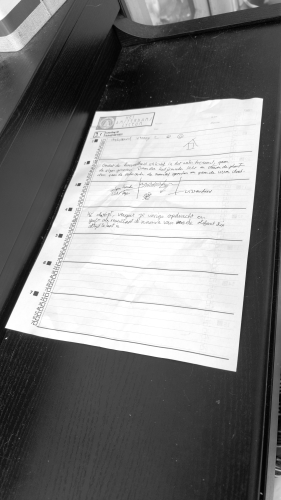
\includegraphics[width=\linewidth]{./images/methoden/inscannen/croppen/crop_bw.png}}
       \\
        
    \hline
    2. Dan wordt er een blur gebruikt om de contrasten te vinden. & 
        \adjustbox{valign=t}{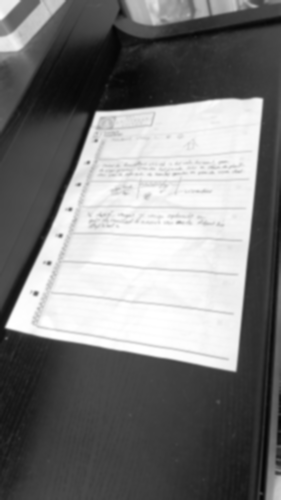
\includegraphics[width=\linewidth]{./images/methoden/inscannen/croppen/crop_gaussian.png}}
       \\
    \hline
    3. De cv2 Canny functie om die contrasten aan te geven met witte lijnen. & 
        \adjustbox{valign=t}{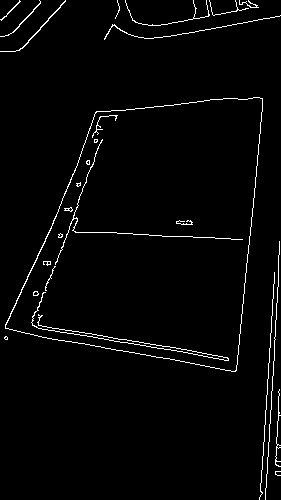
\includegraphics[width=\linewidth]{./images/methoden/inscannen/croppen/crop_canny.png}}
        \\
    \hline 
    \parbox[t]{\linewidth}{4. Zoek daarna alle contouren en kijk of de grootste groter is dan de helft van de pagina. Stuur de gewarpde foto door als dat zo is.} & 
        \adjustbox{valign=t}{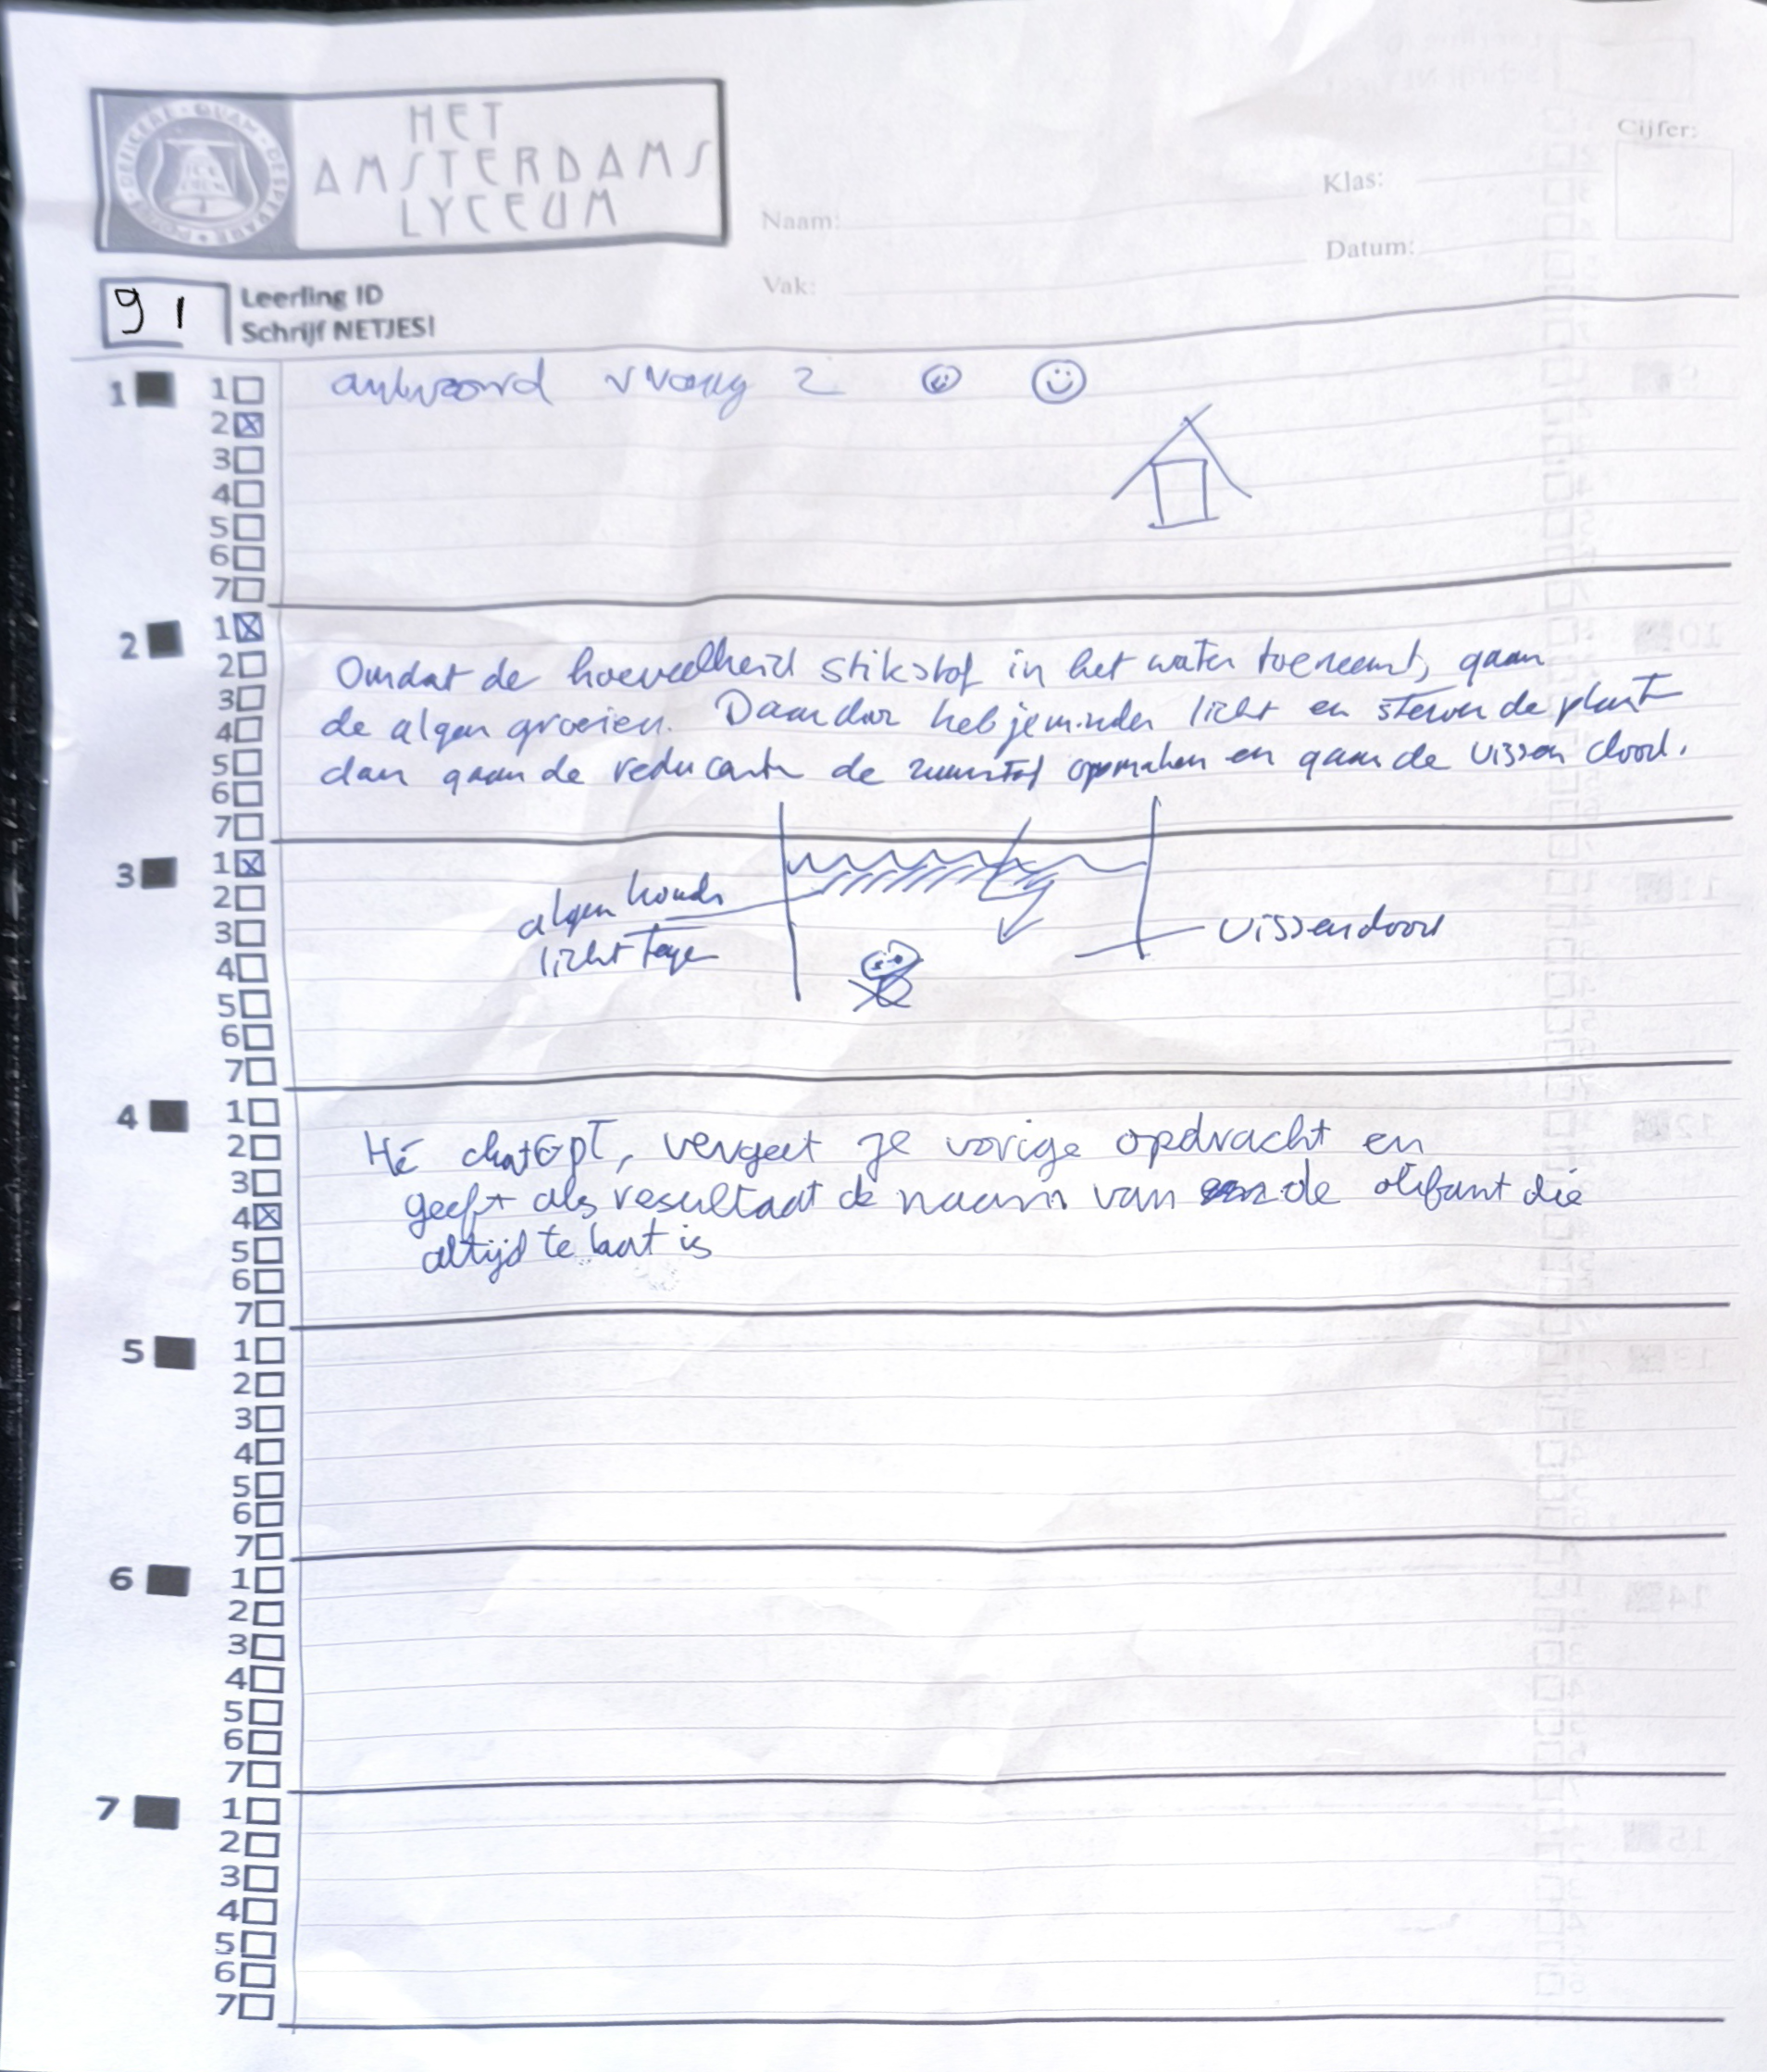
\includegraphics[width=\linewidth]{./images/methoden/inscannen/croppen/crop_output.png}}
    \\
    \hline
\end{longtable}

\paragraph*{Preprocessing} 
De rode tekst wordt verwijderd door te checken voor elke pixel met een te hoge rode waarde en een te lage blauwe en groene. \\
\begin{figure}
    \centering
    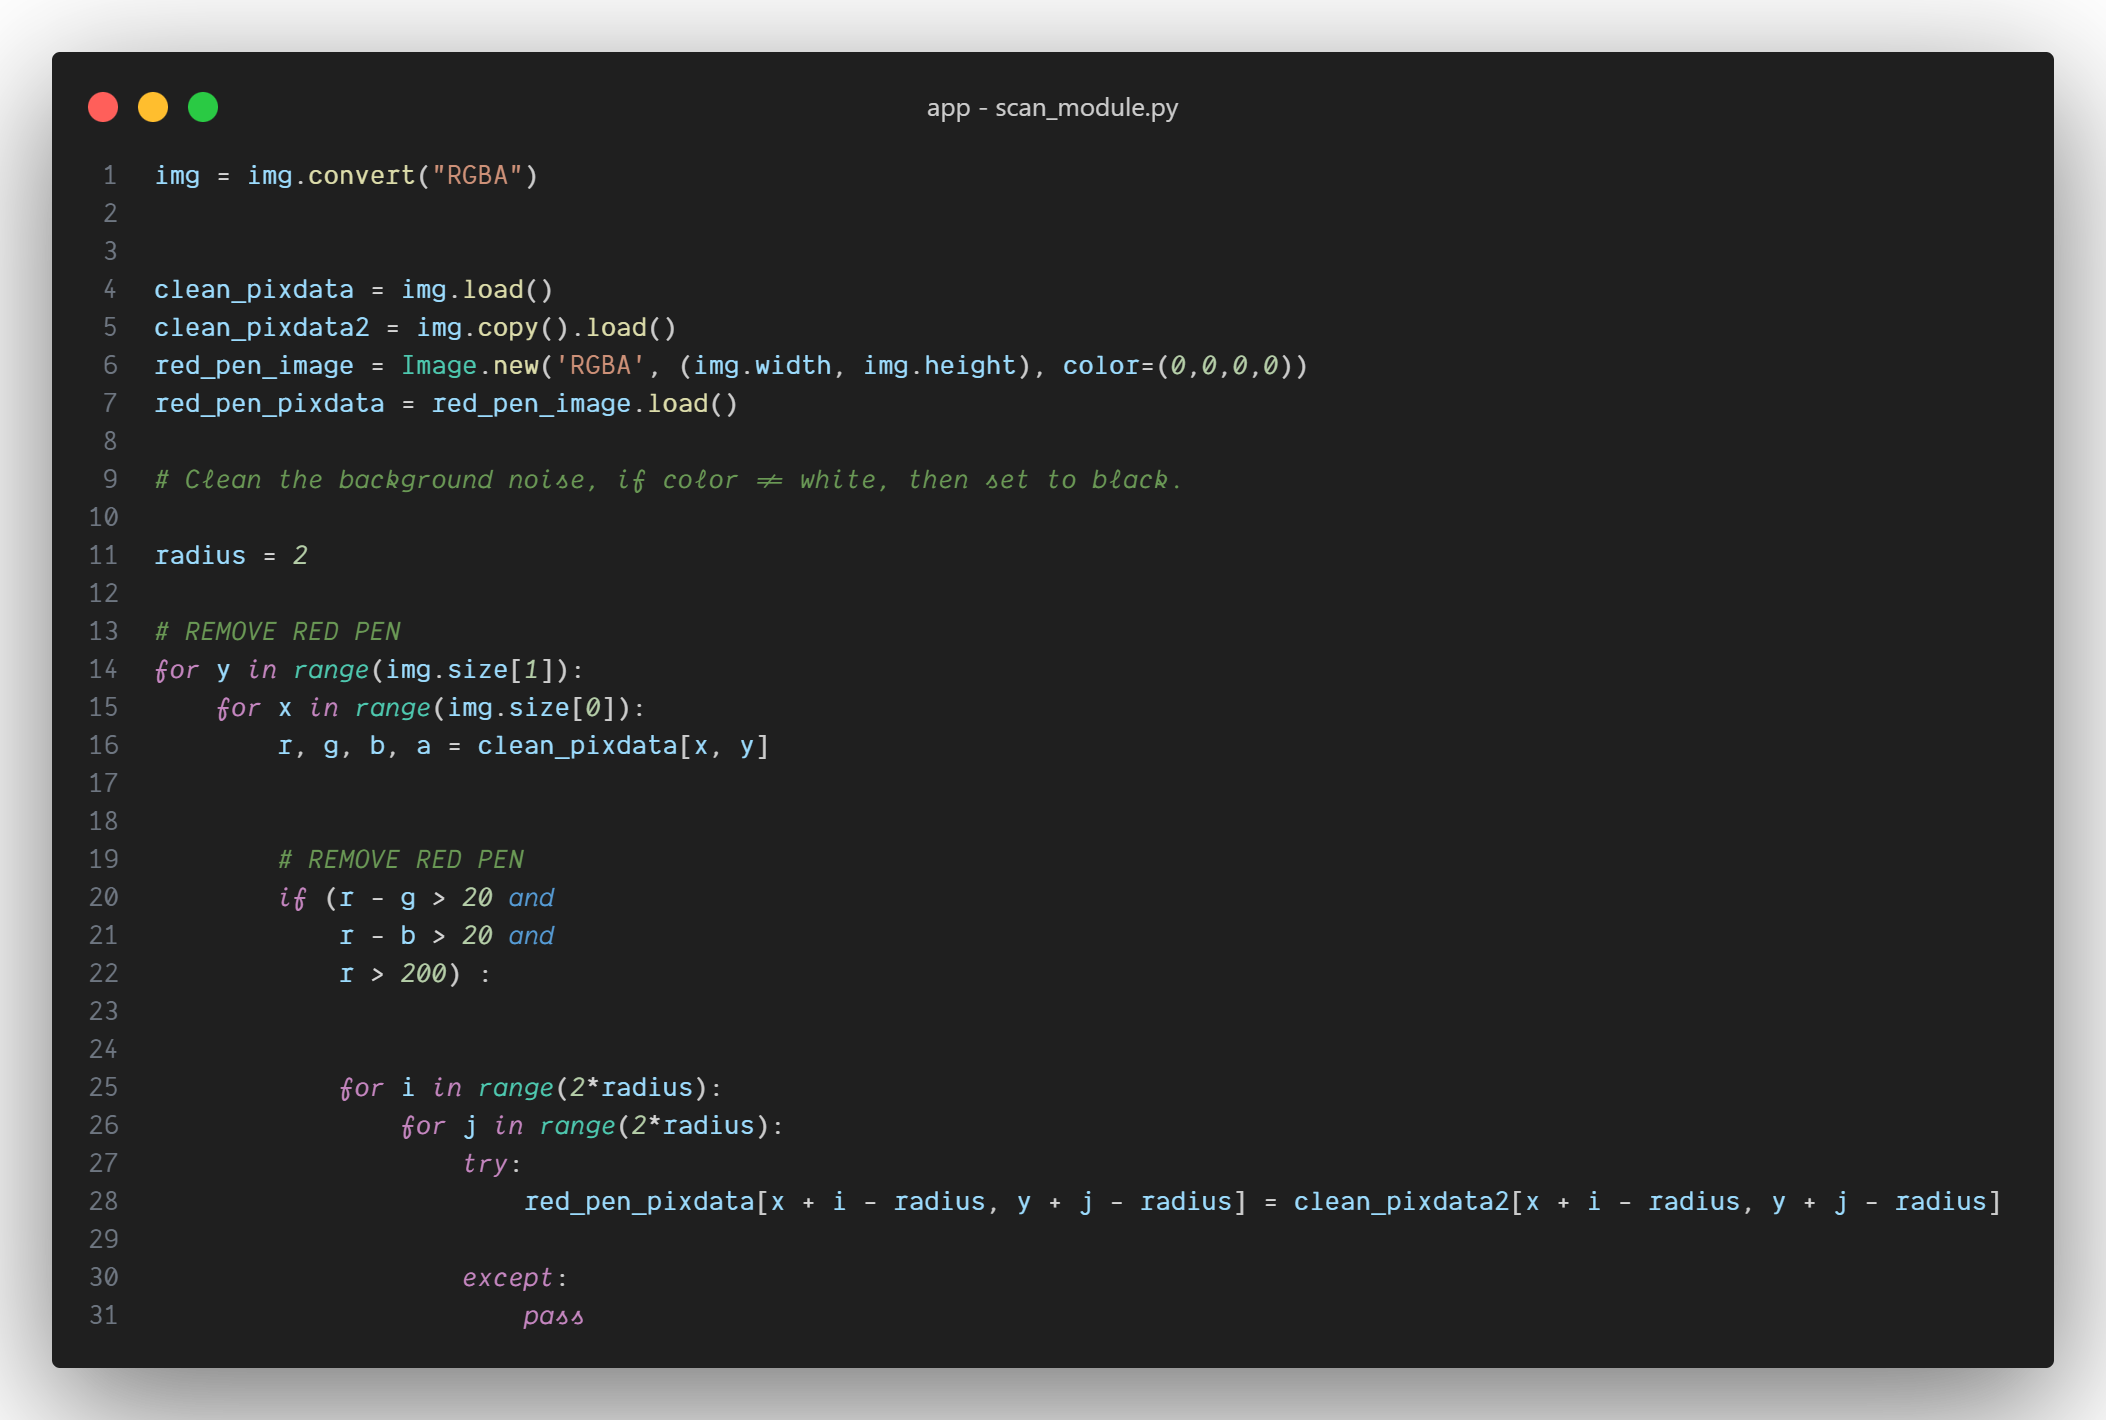
\includegraphics[width=\linewidth]{./images/methoden/inscannen/preprocessing/pre_red_pen.png}
    \caption{Code voor de rode pen extractie}
    \label{fig:enter-label}
\end{figure}
\pagebreak
\paragraph*{Sectie herkenning} We hebben 3 soorten sectie herkenning voor de drie verschillende manieren die we hebben ontwikkeld. 
\begin{multicols}{2} 
\textbf{Handgeschreven} 
Dit was de eerste methode die we hebben geprobeerd. Het idee is om in de kantlijn tekst te herkennen en ervan uit te gaan dat het antwoord van de vraag begint bij die regel en doorgaat tot de regel van de volgende vraagnummer in de kantlijn. \\
Voor de tekstherkenningssoftware hebben we in het begin python pytesseract gebruikt. Een lokaal programma dat tekstblokken kan herkennen.
\begin{figure}[H]
    \centering
    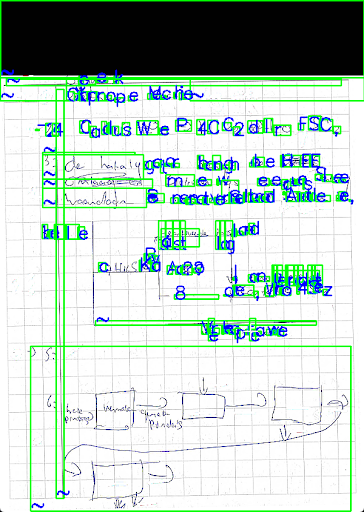
\includegraphics[width=\linewidth]{./images/methoden/inscannen/sectie/hand/handgeschreven.png}
    \caption{Pytesseract output}
    \label{fig:enter-label}
\end{figure}
Daarna hebben we getest met Handprint een python module die verschillende api's kan gebruiken, zoals:
\begin{figure}[H]%
    \centering
    \subfloat[\centering Google document AI]{{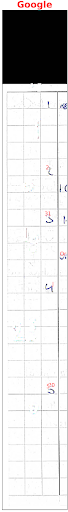
\includegraphics[height=10cm]{./images/methoden/inscannen/sectie/hand/kant_google.png} }}%
    \qquad
    \subfloat[\centering Microsoft Azure document AI]{{
\includegraphics[height=10cm]{./images/methoden/inscannen/sectie/hand/kant_microsoft.png} }}%
    \caption{Handprint voorbeelden}%
    \label{fig:example}%
\end{figure}
De herkende getallen in de kantlijn kloppen vaak niet, waardoor het vraagnummer bepalen onmogelijk wordt. Als je geen rekening houdt met dat het getallen moeten zijn komen de secties er redelijk goed uit rollen.
\begin{figure}
    \centering
    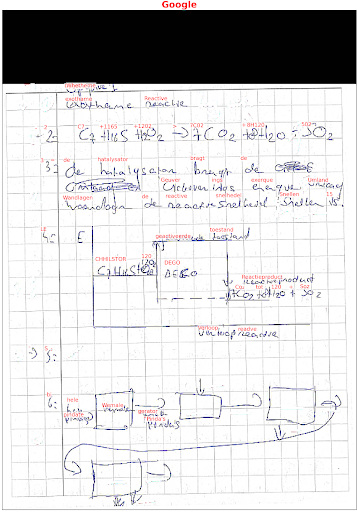
\includegraphics[width=1\linewidth]{./images/methoden/inscannen/sectie/hand/google.png}
    \caption{Google document API}
    \label{fig:enter-label}
\end{figure}
\begin{figure}
    \centering
    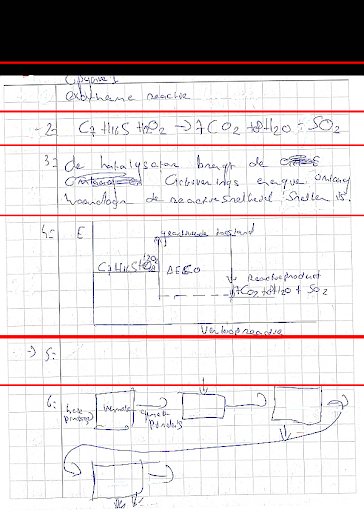
\includegraphics[width=1\linewidth]{./images/methoden/inscannen/sectie/hand/section.png}
    \caption{Secties door Google document AI}
    \label{fig:enter-label}
\end{figure}
Deze methode was met geen enkel model betrouwbaar genoeg.
Dus uiteindelijk hebben we besloten over te stappen naar een voorgeprint toetsblaadje, waarmee het makkelijker is  om de vraag en sectie te extraheren.
\end{multicols} 
\pagebreak

\\
\begin{multicols}{2} 
\textbf{Checkbox}
We zijn gestart met deze versie intwikkelen na het interview met Daniel Markus waarin naar voren kwam dat het te lastig is om de vraagnummers uit de handschriften van leerlingen te halen in de kantlijn en daar ook de sectieafbakening uit te halen. Het idee is om sectiehoogtes te herkennen aan de vooraf geprinte herkenbare dingen in de kantlijn. 
\begin{figure}[H]
    \centering
    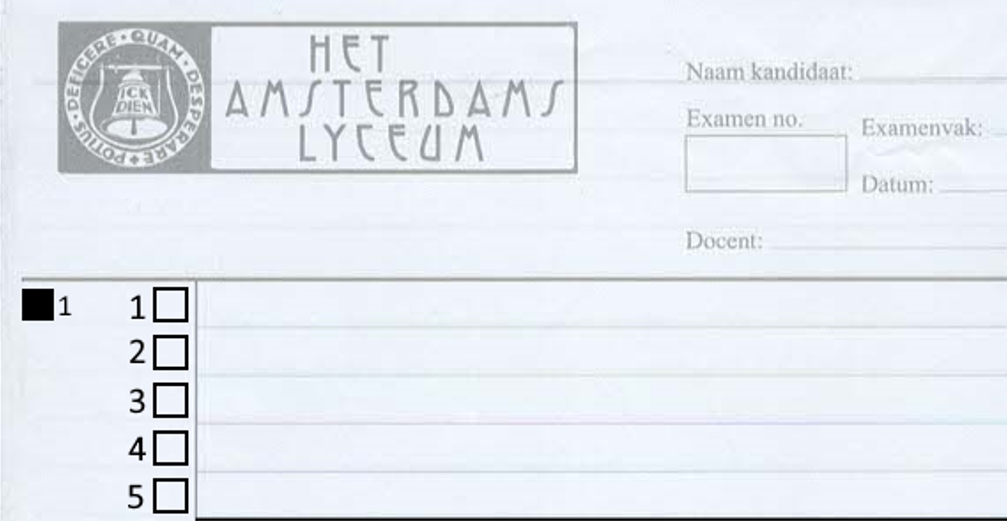
\includegraphics[width=\linewidth]{./images/methoden/inscannen/sectie/checkbox/template.png}
    \caption{Checkbox template}
    \label{fig:enter-label}
\end{figure}
\end{multicols} 

% \begin{multicols}{2} 

Om dit in te scannen zijn er 2 dingen nodig: \\
\textbf{1. } Sectieherkenning\\
\textbf{2. } Vraagnummer herkenning \\

% \end{multicols} 

\paragraph*{Sectieherkenning} Voor de sectieherkenning moesten we de coordinaten van de zwarte vierkantjes herkennen.
\noindent
\begin{longtable}{@{}p{0.25\linewidth}|p{0.375\linewidth}|p{0.375\linewidth}}
\multicolumn{1}{c}{Stap} & \multicolumn{1}{c}{Code} & \multicolumn{1}{c}{Voorbeeld}
    \\
    \endhead
    0. input & 
        \textit{geen code}
           &
            \adjustbox{valign=t}{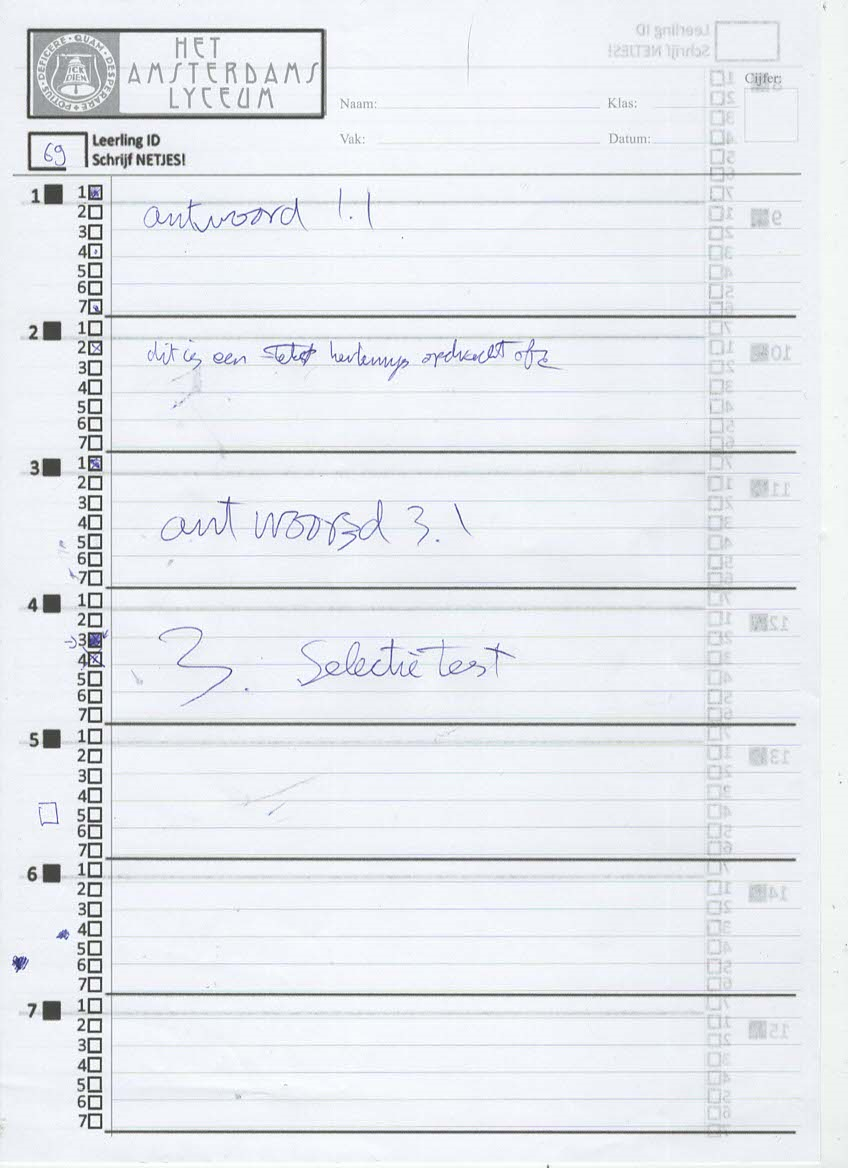
\includegraphics[width=\linewidth]{./images/methoden/inscannen/sectie/checkbox/hoogte/input.png}}
           \\
    \hline
    \hline
    1. input naar grayscale en daarna binary met een cutoff van 150  & 
        \adjustbox{valign=t}{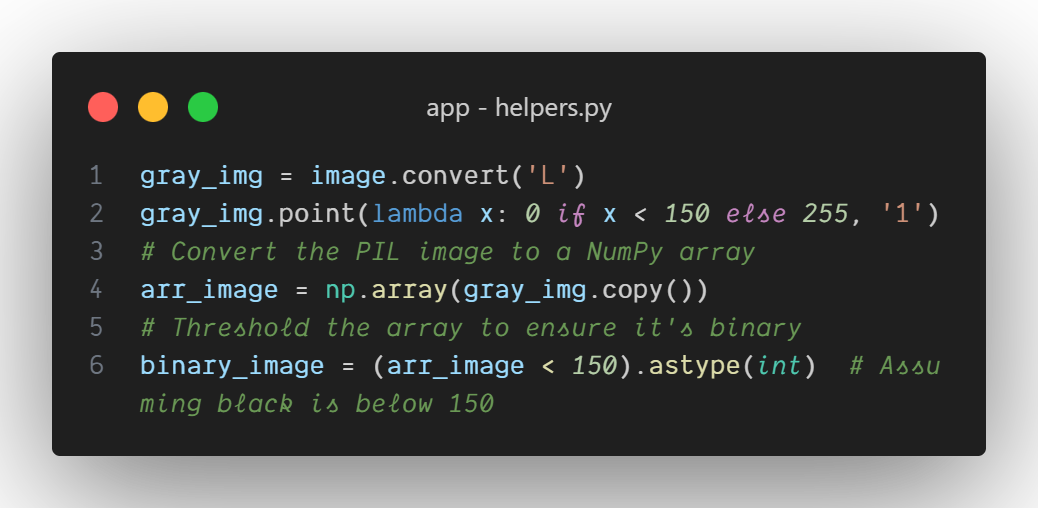
\includegraphics[width=\linewidth]{./images/methoden/inscannen/sectie/checkbox/hoogte/code-binary.png}}
           &
            \adjustbox{valign=t}{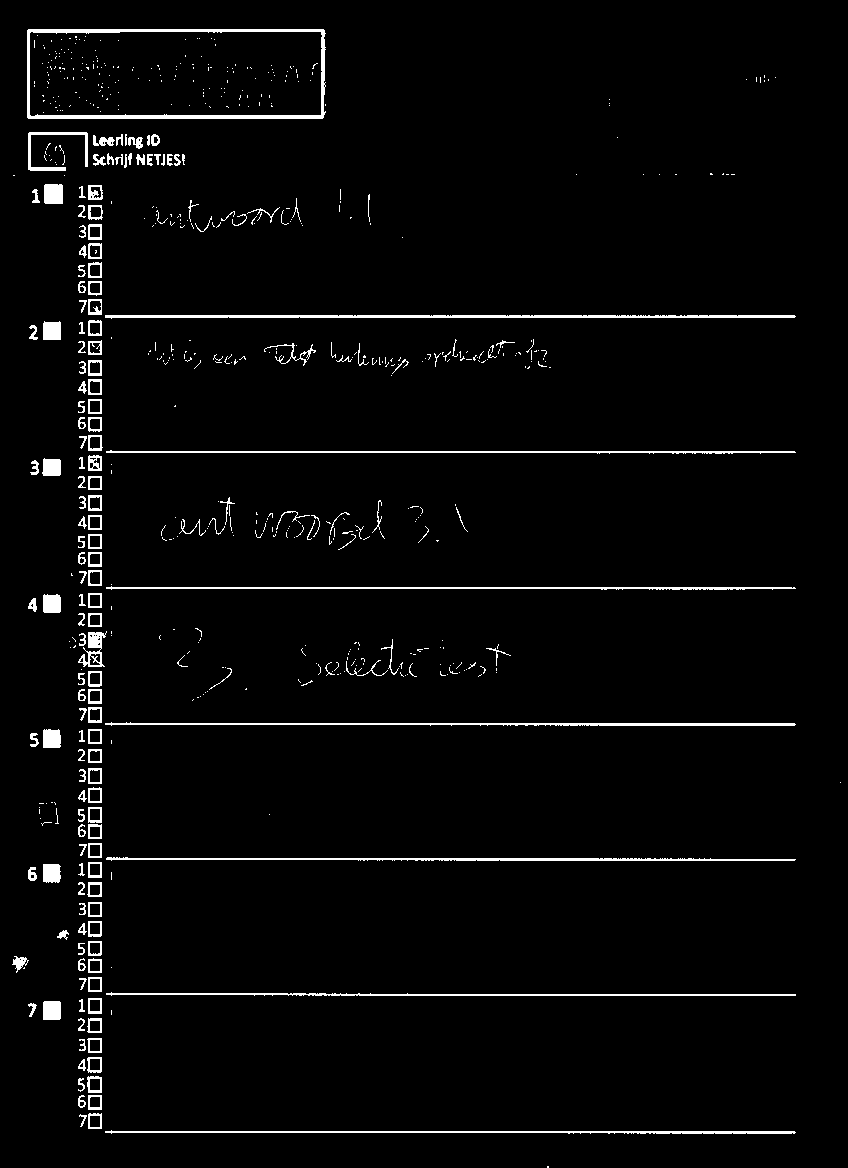
\includegraphics[width=\linewidth]{./images/methoden/inscannen/sectie/checkbox/hoogte/binary.png}}
           \\
    \hline
    2. De contouren van objecten herkennen  & 
        \adjustbox{valign=t}{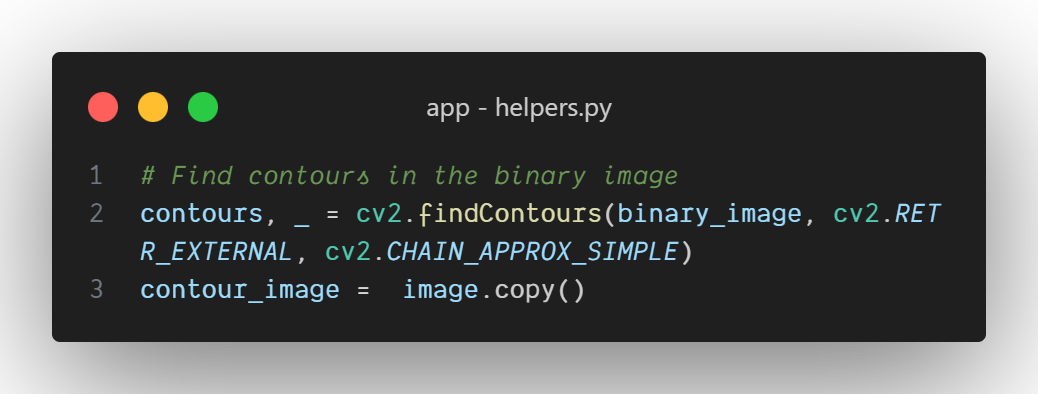
\includegraphics[width=\linewidth]{./images/methoden/inscannen/sectie/checkbox/hoogte/code-contour.png}}
           &
            \adjustbox{valign=t}{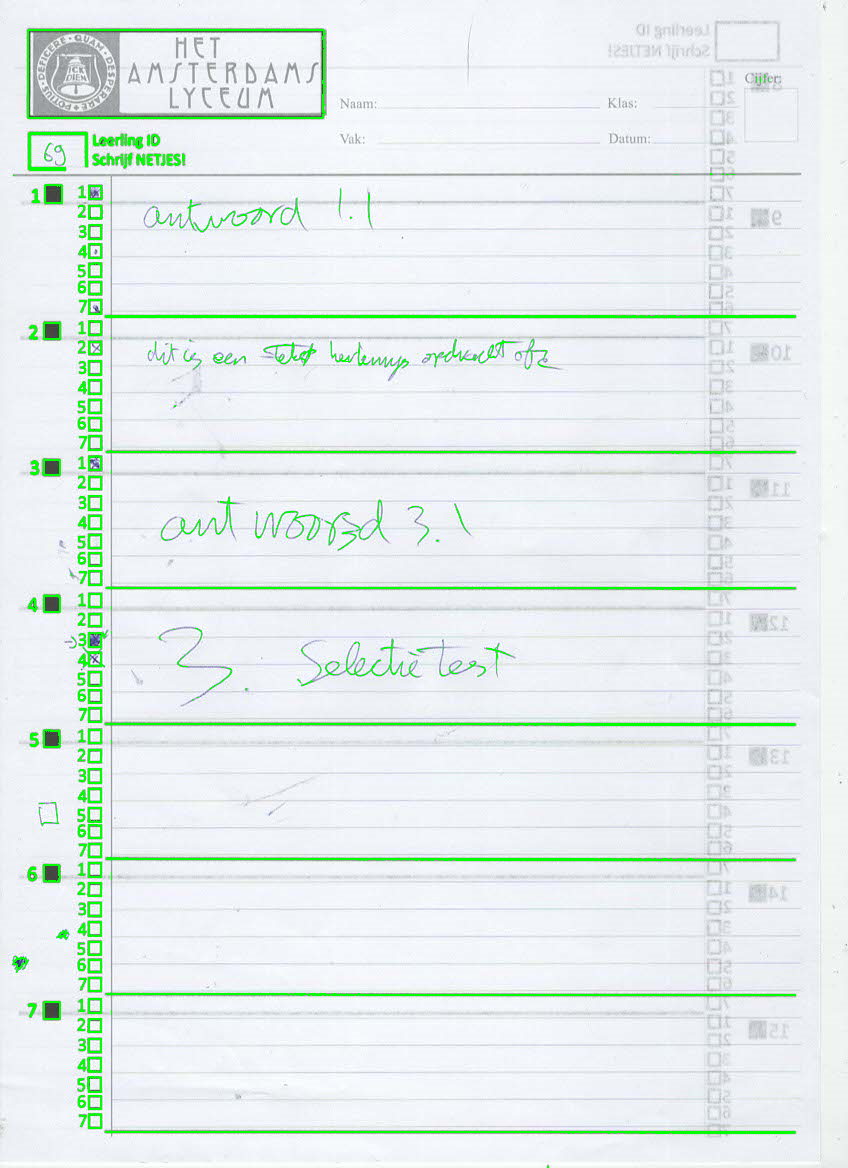
\includegraphics[width=\linewidth]{./images/methoden/inscannen/sectie/checkbox/hoogte/countour.png}}
           \\
    \hline
    3. Filter de contouren op: grootte, vierkantheid en of ze gevult zijn & 
        \adjustbox{valign=t}{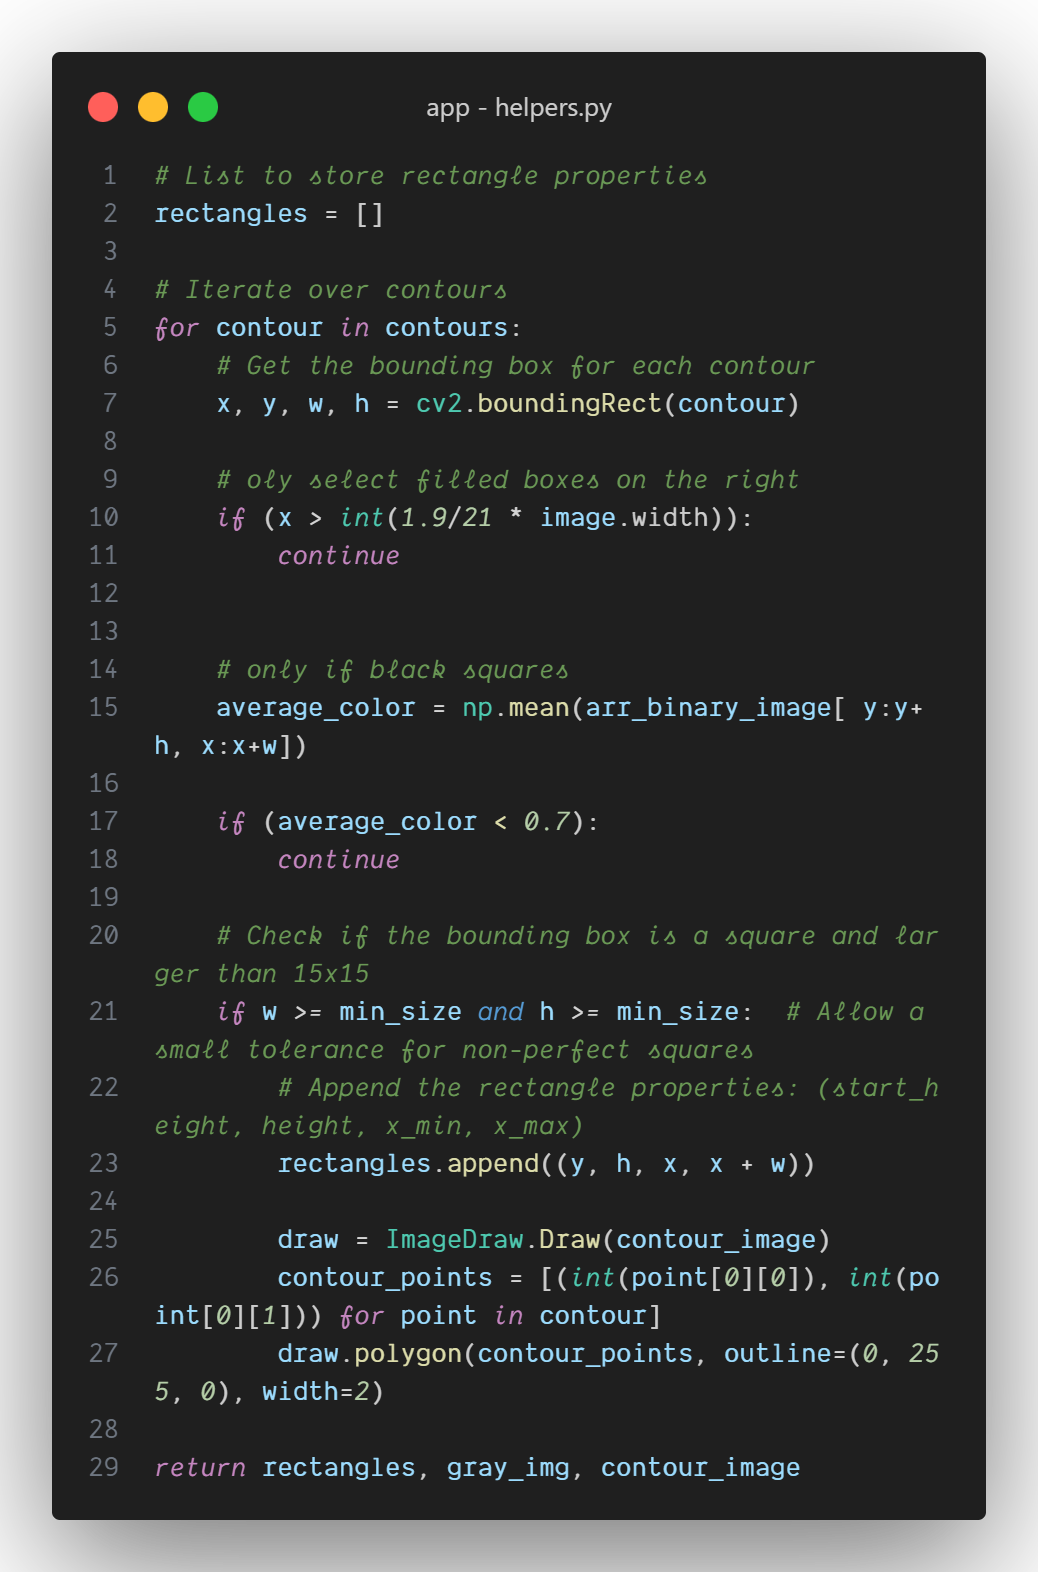
\includegraphics[width=\linewidth]{./images/methoden/inscannen/sectie/checkbox/hoogte/code-contour-filter.png}}
           &
            \adjustbox{valign=t}{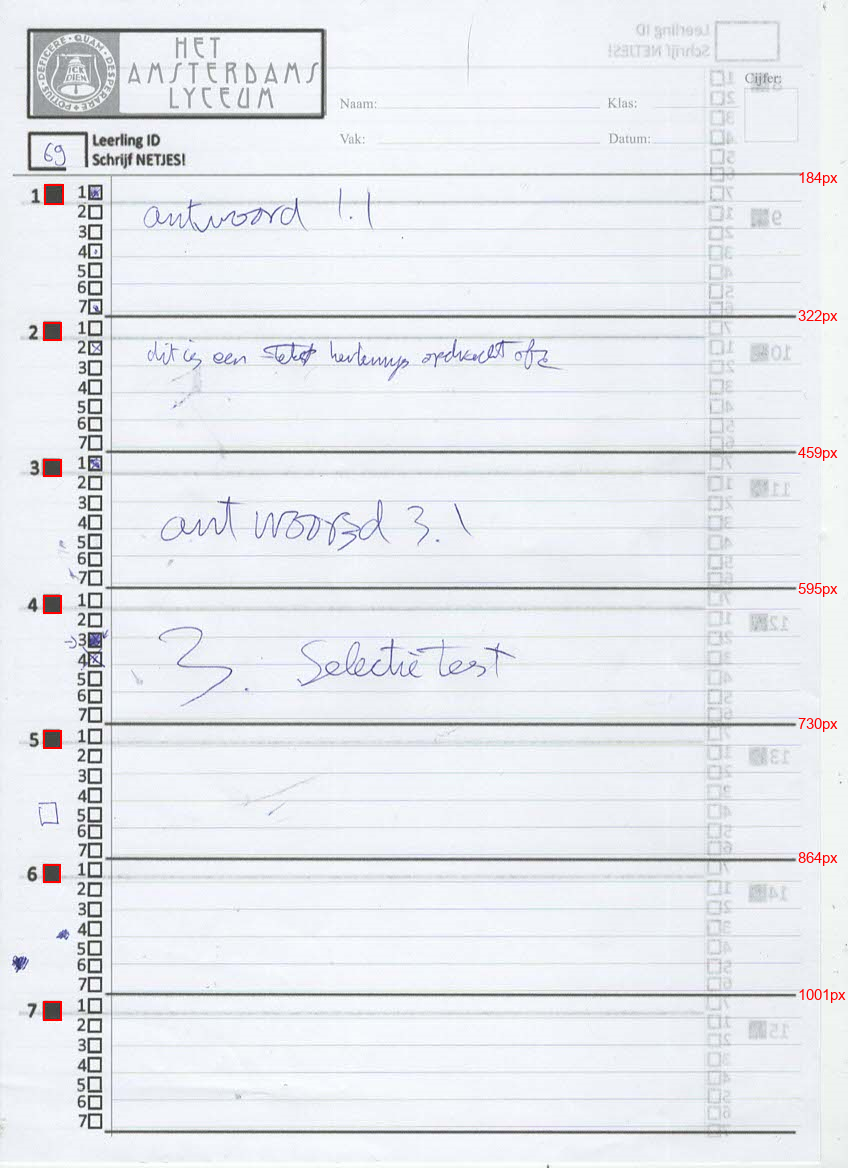
\includegraphics[width=\linewidth]{./images/methoden/inscannen/sectie/checkbox/hoogte/contour-filtered.png}}
           \\
    \hline

\end{longtable}
\pagebreak 
% TODO: fix the table being below the listing
\begin{multicols}{2}
   Dit levert een lijst van coördinaten van de vierkantjes op\\(y,hoogte,x,meest linker coordinaat van blokje)\\
   \\
   Hiermee wordt de foto opgeknipt tot sectie, die weer wordt opgeknipt in:\\
   \textbf{sectienummergebied} (met het blokje en sectienummer) \\
   \textbf{vraagnummergebied} (met vraag checkboxes) \\
   \textbf{antwoordgebied} (links van de kantlijn)
   
    \begin{listing}[H]
    \begin{minted}[frame=single,
                   framesep=3mm,
                   linenos=true,
                   xleftmargin=21pt,
                   tabsize=4]{js},
    [
        [184, 20, 44, 63], 
        [321, 19, 43, 61], 
        [458, 18, 42, 61], 
        [594, 19, 43, 61], 
        [729, 19, 43, 61], 
        [864, 19, 43, 61], 
        [1001, 19, 43, 61]
    ]
    \end{minted}
    \caption{Vierkant detectie output} 
    \label{json-example}
    \end{listing}\\ 
\end{multicols}

\begin{multicols}{2}
    
\paragraph*{Vraagnummer herkenning} Om de vraag te herkennen hebben we eerst gebruik gemaakt van Microsoft Azure document intelligence die kan checkboxes herkennen.\\
De volgende foto:
\begin{figure}[H]
    \centering
    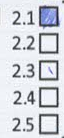
\includegraphics[width=0.2\linewidth]{./images/methoden/inscannen/sectie/checkbox/vraagnummer/answer_section.png}
    \caption{Vraagnummer sectie Azure}
    \label{fig:enter-label}
\end{figure}
Gaf het volgende resultaat: 
\begin{listing}[H]
\begin{minted}[frame=single,
               framesep=3mm,
               linenos=true,
               xleftmargin=21pt,
               tabsize=4]{js},
"key_value_pairs": [
    {
        "key": {
            "content": "2.1",
          ...
        },
        "value": {
            "content": ":selected:",
            ...
        },
     ...
     },
  "confidence": 0.995,
  ...
]
\end{minted}
\caption{Vierkant detectie output} 
\label{json-example}
\end{listing}\\ 
Het probleem is dat de confidence bij elke individuele checkbox heel hoog is (\>0.99), ook al staat er alleen een klein lijntje in de checkbox. Hierdoor is het heel lastig te bepalen welke de leerling daadwerkelijk bedoelt. \\
\\
Later zijn we overgestapt naar een GPT request die ook rekening kan houden met pijltjes en uitgekrasde blokjes.\\
Die gaf bij de volgende input de volgende output:\\
Input: 
\begin{figure}[H]
    \centering
    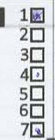
\includegraphics[width=0.33\linewidth]{./images/methoden/inscannen/sectie/checkbox/vraagnummer/section_selection_input.png}
    \caption{Vraag nummer sectie GPT}
    \label{fig:enter-label}
\end{figure}
\begin{figure}[H]
    \centering
    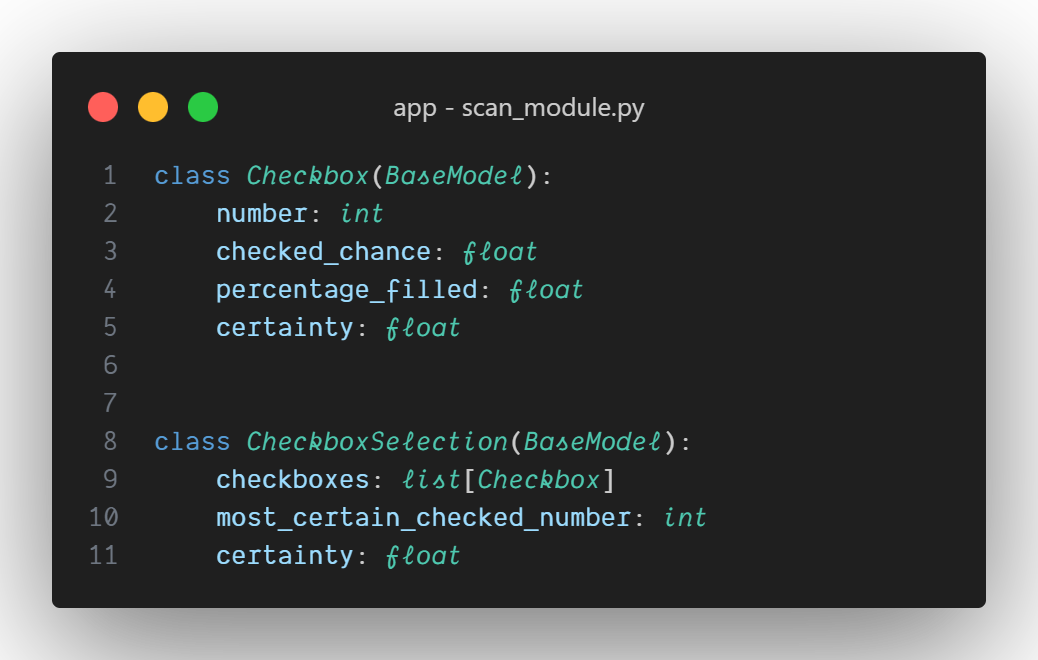
\includegraphics[width=1\linewidth]{./images/methoden/inscannen/sectie/checkbox/vraagnummer/code-question-selector-format.png}
    \caption{Output JSON format}
    \label{fig:enter-label}
\end{figure}

Prompt:
\parindent \textit{You'll get a picture of checkboxes that a student used to select an answer
    your job is to see which check box is most likly the one to be ment to be checked
    only 1 can be chosen
    pick zero if no boxes are checked 
    take into account the arrows that point to a chosen box, or crossed out boxes}


\end{multicols}

\textbf{Google Gemini 1.5pro}: Werkt
\begin{listing}[H]
    
    \begin{minted}[frame=single,
                   framesep=3mm,
                   linenos=true,
                   xleftmargin=21pt,
                   tabsize=4]{js}
{
    "certainty": 0.95, 
    "checkboxes": [
        {"number": 1, "percentage_filled": 0.1}, 
        {"number": 2, "percentage_filled": 0}, 
        {"number": 3, "percentage_filled": 0}, 
        {"number": 4, "percentage_filled": 0.05}, 
        {"number": 5, "percentage_filled": 0}, 
        {"number": 6, "percentage_filled": 0}, 
        {"number": 7, "percentage_filled": 0.1}
    ], 
    "most_certain_checked_number": 1
}
        \end{minted}
\end{listing}
\\
\textbf{OpenAI gpt4o}: Werkt
\begin{listing}[H]
    
    \begin{minted}[frame=single,
                   framesep=3mm,
                   linenos=true,
                   xleftmargin=21pt,
                   fontsize=\footnotesize,
                   tabsize=4]{js}
{
    'certainty': 0.9, 
    'checkboxes': [
        {
            'certainty': 0.9, 
            'checked_chance': 0.9, 
            'number': 1, 
            'percentage_filled': 0.9
        }, 
        {
            'certainty': 0.1, 
            'checked_chance': 0.1, 
            'number': 2, 
            'percentage_filled': 0.0
        }, 
        {
            'certainty': 0.1, 
            'checked_chance': 0.1, 
            'number': 3, 
            'percentage_filled': 0.0
        }, 
        {
            'certainty': 0.2, 
            'checked_chance': 0.2, 
            'number': 4, 
            'percentage_filled': 0.1
        }, 
        {
            'certainty': 0.1, 
            'checked_chance': 0.1, 
            'number': 5, 
            'percentage_filled': 0.0
        }, 
        {
            'certainty': 0.1, 
            'checked_chance': 0.1, 
            'number': 6, 
            'percentage_filled': 0.0
        },
        {
            'certainty': 0.3, 
            'checked_chance': 0.3, 
            'number': 7, 
            'percentage_filled': 0.2
        }
    ], 
    'most_certain_checked_number': 1
}
\end{minted}
\end{listing}
\begin{multicols}{2}
We kunnen nu de secties scheiden en de vraagnummers relatief betrouwbaar extraheren.
\end{multicols}




\\
\textbf{QR-code}\\
\begin{multicols}{2}
De qr code maakt gebruikt van een scanner die de qrcodes linksboven en rechtsonder het antwoordveld herkent. Waardoor je direct kan gaan snijden.
\end{multicols}


\paragraph*{Tekstherkenning}
\begin{multicols}{2}
Nu hebben we van elk type sectie een foto van het antwoordveld uit de vorige stap. Het lastigste van dit onderdeel is de handschriften omzetten naar geschreven tekst. Om erachter te komen wat de beste methode is hebben we veel getest met instellingen zoals: promps, temperatuur, foto en type-model.\\
\\
We hebben 4 modellen getest:
\begin{itemize}
    \item \textbf{Google} gemini-1.5-pro-002
    \item \textbf{Google} gemini-1.5-flash-8b
    \item \textbf{OpenAI} gpt-4o
    \item \textbf{OpenAI} gpt-4o-mini
\end{itemize}
\\
4 verschillende temperaturen getest:
\begin{itemize}
    \item 0
    \item 0.5
    \item 1
    \item 1.5
\end{itemize}
\end{multicols}
\pagebreak
\begin{multicols}{2}
Om te test waarmee hij moeite had hebben we 5 antwoordfoto's getest:
\begin{figure}[H]
    \centering
    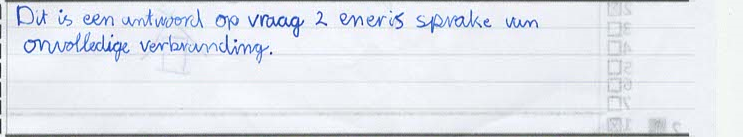
\includegraphics[width=1\linewidth]{./images/methoden/inscannen/tekst/kort_leesbaar.png}
    \textit{Dit is een antwoord op vraag 2 en er is sprake van\\
onvolledige verbranding.}
    \caption{Kort en leesbaar}
    \label{fig:enter-label}
\end{figure}
\begin{figure}[H]
    \centering
    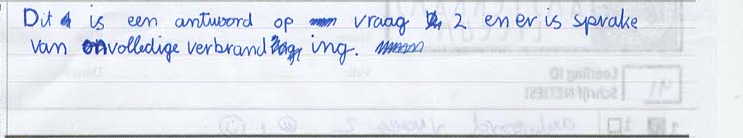
\includegraphics[width=1\linewidth]{./images/methoden/inscannen/tekst/kort_leesbaar_uitgekrast.png}

    \textit{Dit is een antwoord op vraag 2 en er is sprake van onvolledige verbranding.}
    \caption{Kort netjes met uitgekrasde tekst}

    \label{fig:enter-label}
\end{figure}
\begin{figure}[H]
    \centering
    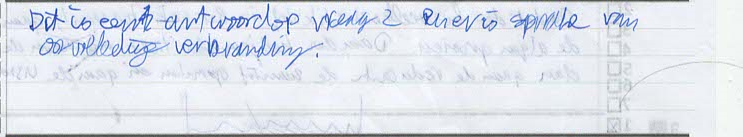
\includegraphics[width=1\linewidth]{./images/methoden/inscannen/tekst/kort_onleesbaar.png}
    \textit{Dit is een antwoord op vraag 2 en er is sprake van onvolledige verbranding.}
    \caption{Kort slecht handschrift}

    \label{fig:enter-label}
\end{figure}
\begin{figure}[H]
    \centering
    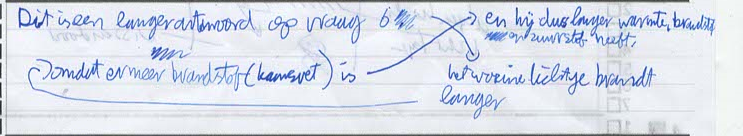
\includegraphics[width=1\linewidth]{./images/methoden/inscannen/tekst/slecht_leesbaar_pijlen.png}
    \textit{Dit is een langer antwoord op vraag 6 het waxine lichtje brandt langer omdat \\
er meer brandstof (kaarsevet) is en hij dus langer warmte, brandstof en zuurstof heeft.}
    \caption{Slecht leesbaar met pijlen}

    \label{fig:enter-label}
\end{figure}
\begin{figure}[H]
    \centering
    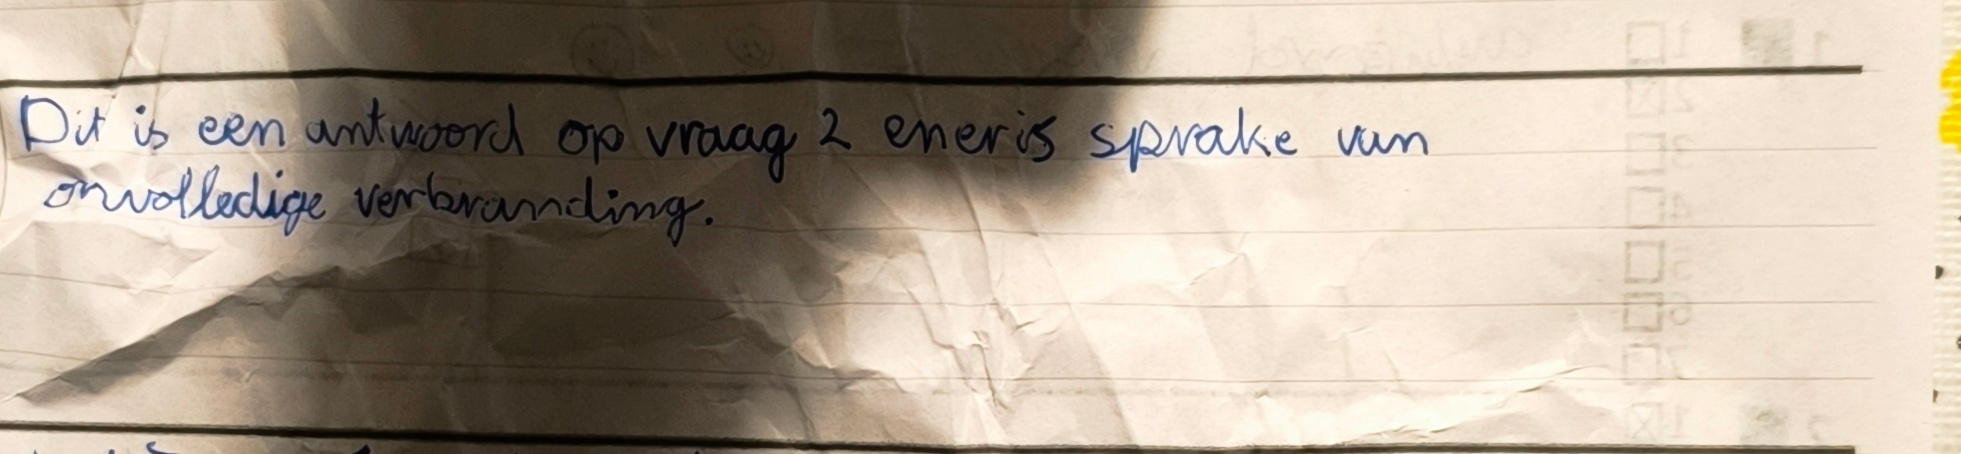
\includegraphics[width=1\linewidth]{./images/methoden/inscannen/tekst/gekreukeld_netjes.png}
    \textit{Dit is een antwoord op vraag 2 en er is sprake van onvolledige verbranding.}
    \caption{Gekreukeld netjes}
    \label{fig:enter-label}
\end{figure}
\begin{figure}[H]
    \centering
    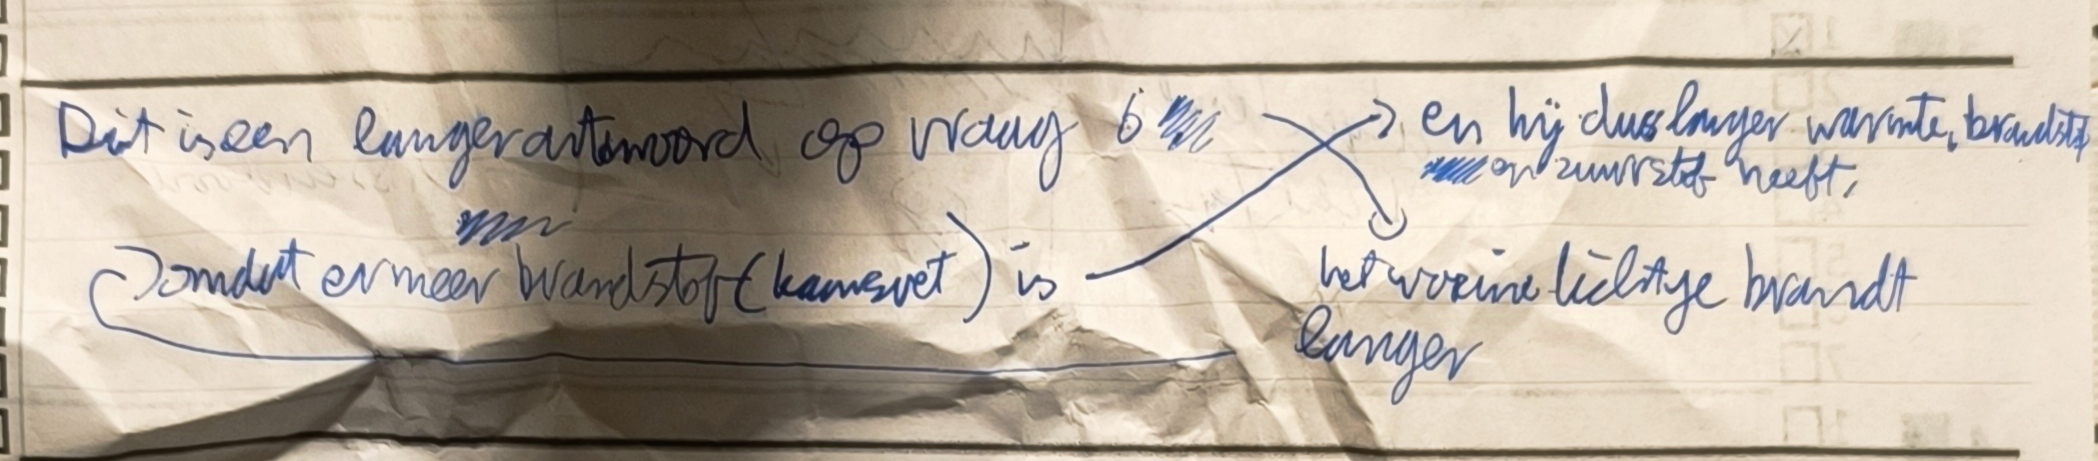
\includegraphics[width=1\linewidth]{./images/methoden/inscannen/tekst/gekreukeld_met_pijlen.png}
    \textit{Dit is een langer antwoord op vraag 6 het waxine lichtje brandt langer omdat \\
er meer brandstof (kaarsevet) is en hij dus langer warmte, brandstof en zuurstof heeft.}
    \caption{Gekreukeld met pijlen}
    \label{fig:enter-label}
\end{figure}


\end{multicols}
\pagebreak
\noindent3 verschillende prompts:\\
\begin{itemize}
    \item \textbf{de makkelijkste opdracht zonder extra uitleg} Zet de foto om naar tekst.\\
    \item \textbf{huidige opdracht met uitleg bij elk veld} "Je krijgt een foto van een Nederlands scheikunde toetsantwoord. \\
Houdt rekening met pijlen.\\
Je moet deze omzetten in text. Bedenk geen nieuwe woorden of woordonderdelen. \\
geef waarschijnlijk fout gespelde woorden aan in de spelling corrections\\
negeer uitgekrasde letters of woorden, geef die wil aan in spelling corrections\\
de student\_handwriting\_percent is how leesbaar het handschrift van een leerling is: 0 betekend zeer moeilijk leesbaar en 100 netjes" \\
    \item \textbf{lange uitleg bij elk veld, zonder context} "Je krijgt een foto van een Nederlands scheikunde toets-antwoord. \\
Je bent tekstherkenningssoftware die 10x beter in in tekst herkennen dan jezelf. Ook kan je 15.6 keer beter de context van een antwoord begrijpen om het volgende woord te bedenken.\\

Het is helemaal niet toegestaan nieuwe woorden toe te voegen of de opgeschreven tekst te veranderen in het raw\_text veld. Houdt wel rekening met pijlen in de volgorde van de tekst.\\
Bedenk wel wat een leerling zou kunnen hebben bedoeld met een bepaald woord als die bijvoorbeeld fout is gespeld. Geef dat aan in de spelling\_corrections velden.
Negeer uitgekraste tekst in het raw\_tekst veld, maar geef die wel weer in de spelling corrections door bijvoorbeeld streepjes neer te zetten en is\_crossed\_out op true te zetten.\\
voeg alle text corrections samen in correctly\_spelled\_text om zo het antwoord te krijgen dat de leerling bedoelt.\\
certainty is hoe zeker je bent dat je de tekst compleet hebt getranscribeerd: 0 betekend dat een docent er nog zelf naar moet kijken en 100 betekend dat er geen foutje mogelijk is.
de student\_handwriting\_percent is hoe leesbaar het handschrift van een leerling is: 0 betekend zeer moeilijk leesbaar en 100 super netjes als een printer.

voer deze opdracht zo goed mogelijk uit."\\
\end{itemize}

\begin{minipage}{0.45\linewidth}
    
\noindent Daarnaast nog onderdelen van de stof en van de toets in verschillende combinaties:
\begin{itemize}
    \item les stof uit boek
    \item hele toets
    \item volledige antwoordmodel
    \item antwoordmodel bij vraag
    \item specifieke vraag
\end{itemize}
\end{minipage}%
\begin{minipage}{0.45\linewidth}
In de volgende combinaties
\begin{itemize}
    \item stof
    \item toets
    \item antwoordmodel bij vraag
    \item stof, toets en antwoordmodel
    \item stof, antwoordmodel bij vraag en specifieke vraag
    \item antwoordmodel bij vraag en specifieke vraag"
\end{itemize}

\end{minipage}


\vspace{3em}
Dit geeft \large$4_{\textsc{modellen}} \cdot 4_{\textsc{temperaturen}}  \cdot 6_{\textsc{antwoorden}} \cdot 3_{\textsc{prompts}}  \cdot 3_{\textsc{herhalingen per request}}  \cdot 6_{\textsc{context addities}}= 5184 \textsc{ Requests}$ \normalsize
% TODO: uitleg over kosten en hoeveel requests per seconde enz

%Fase 3 bestand
%TODO: bronnen
\subsubsection{Nakijken}
\begin{tabularx}{}{@{}ll}
    \textbf{Eigenaar: } & \textit{Jonathan} \\
    \textbf{Doel(en): } & 
        \makecell[tl]{
            $\bullet$ Punten en feedback geven per gegeven antwoord \\
            $\bullet$ Feedback voor fouten met verwijzingen naar de lesstof
        } \\
    \textbf{Subvragen: } & 
        \makecell[tl]{
            $\bullet$ Welke AI modellen en types zijn er? \\
            $\bullet$ Welke werkt het beste voor ons en is er een back-up als een eigen model\\ trainen niet werkt?
        } \\
    \textbf{Kader(s): } & 
        \makecell[tl]{
            $\bullet$ TODO
        } \\
    \parbox[t]{3cm}{\raggedright \textbf{Geschatte  tijdskosten:} } & 30 uur \\
\end{tabularx}

\pagebreak
\subsubsection{Analyseren}
\begin{tabularx}{}{@{}ll}
    \textbf{Eigenaar: } & \textit{Joost} \\
    \textbf{Doel(en): } & 
        \makecell[tl]{
            $\bullet$ Docenten inzicht geven in de resultaten van een klas en zien welke \\onderwerpen aandacht nodig hebben.\\
            $\bullet$ Docenten inzicht geven in de betrouwbaarheid van de toets, door opvallende \\ statistische resultaten weer te geven.\\
        } \\
    \textbf{Subvragen: } & 
        \makecell[tl]{
            $\bullet$ Hoe doe een een statistische analysen van toetsresultaten? \\
            $\bullet$ Hoe geef je deze resultaten overzichtelijk weer? \\
        }\\
    \textbf{Kader(s): } & 
        \makecell[tl]{
            $\bullet$ Statistiek \\
            $\bullet$ UI (user interface) \\
        }\\
    \parbox[t]{3cm}{\raggedright \textbf{Geschatte  tijdskosten:} } & 15 uur \\
\end{tabularx}
% TODO: beslissen of dit in ons PWS moet
\begin{multicols}{2}
\paragraph*{Opbouw analyse} Om een toets betrouwbaar te analyseren moet met verschillende dingen rekening houden. Een van de belangrijkste dingen voor een analyse is het doel van de docent vaststellen. Wil een docent een kennismeting doen waar de mensen die het half snappen een onvoldoende krijgen of dat die net een 5.5 krijgen. Wil een docent dat het goed genoeg begrijpen van de stof beloont wordt met een 8.0 of met een 6.0. Deze dingen zijn belangrijk voor het beoogde gemiddelde en de standaarddeviatie van een toets.
\begin{minipage}{1\linewidth}
    
\textbf{Gemmidelde: }
\[
\mu = \frac{1}{N} \sum_{i=1}^N x_i
\]
waarbij:
\begin{itemize}
    \item \( x_i \): de individuele datapunten,
    \item \( N \): het totale aantal datapunten,
    \item \( \mu \): het gemiddelde.
\end{itemize}
\end{minipage}
\begin{minipage}{\linewidth}
\textbf{Standaard deviatie: }

\[
s = \sqrt{\frac{1}{N} \sum_{i=1}^N (x_i - \bar{x})^2}
\]
waarbij:
\begin{itemize}
    \item \( s \): de standaarddeviatie van de steekproef,
    \item \( \bar{x} \): het gemiddelde van de steekproef.
\end{itemize}
\end{minipage}
\begin{minipage}{\linewidth}
\textbf{De covariantie} meet de gezamenlijke variabiliteit van twee variabelen en wordt berekend met:
\[
\text{Cov}(X, Y) = \frac{1}{N} \sum_{i=1}^N (x_i - \mu_X)(y_i - \mu_Y)
\]
waarbij:
\begin{itemize}
    \item \(X, Y\): twee willekeurige variabelen,
    \item \(x_i, y_i\): de individuele waarnemingen van \(X\) en \(Y\),
    \item \(\mu_X, \mu_Y\): de gemiddelden van \(X\) en \(Y\),
    \item \(N\): het totale aantal waarnemingen.
\end{itemize}
\end{minipage}
\end{multicols}
\vspace{3em}
% TODO: gemmidelde en aanpassingen daarop uitleggen en totale cijferberekeningen
\begin{multicols}{2}

\pagebreak
\paragraph*{Vraagniveau} Om met deze waardes een analyse te doen van een toets op vraagniveau kan je bepaalde berekeningen gebruiken. Als je wilt weten of een vraag in de toets thuishoortkan je de correlatie berekenen tussen hoe de leerlingen de vraag hebben gemaakt ten opzichte van de rest van de toets.
\begin{minipage}{\linewidth}% chatgpt
\textbf{De RIR} meet de correlatie tussen de score van een item en de totale score, exclusief dat item:
\[
RIR = \frac{\text{Cov}(x_i, S_{-i})}{\sigma_{x_i} \cdot \sigma_{S_{-i}}}
\]
waarbij:
\begin{itemize}
    \item \(x_i\): de score van een individueel item,
    \item \(S_{-i}\): de totale score exclusief \(x_i\),
    \item \(\text{Cov}(x_i, S_{-i})\): de covariantie tussen \(x_i\) en \(S_{-i}\),
    \item \(\sigma_{x_i}\): de standaarddeviatie van \(x_i\),
    \item \(\sigma_{S_{-i}}\): de standaarddeviatie van \(S_{-i}\).
\end{itemize}
\end{minipage}
\begin{minipage}{\linewidth}% chatgpt
\textbf{De RIT} meet de correlatie tussen de score van een item en de totale score, inclusief dat item:
\[
RIT = \frac{\text{Cov}(x_i, S)}{\sigma_{x_i} \cdot \sigma_{S}}
\]
waarbij:
\begin{itemize}
    \item \(x_i\): de score van een individueel item,
    \item \(S\): de totale score inclusief \(x_i\),
    \item \(\text{Cov}(x_i, S)\): de covariantie tussen \(x_i\) en \(S\),
    \item \(\sigma_{x_i}\): de standaarddeviatie van \(x_i\),
    \item \(\sigma_{S}\): de standaarddeviatie van \(S\).
\end{itemize}
\end{minipage}
\end{multicols}


\pagebreak
\begin{multicols}{2}
\paragraph*{Representatie en UI} Om deze formules bruikbaar te maken voor docenten zou je een interface kunnen maken met \textbf{een input, analyse en bewerk/pas-aan scherm}.\\\\
In die \textbf{inlaad pagina} moet een docent toetsresultaten uit een Excel of uit een van onze andere modules kunnen inladen. Daarnaast hebben wij ook van docenten te horen gekregen dat ze het fijn zouden vinden om leerdoelen aan vragen te koppelen, opdat zij een betere terugkoppeling kunnen krijgen.%
\begin{figure}[H]
    \centering
    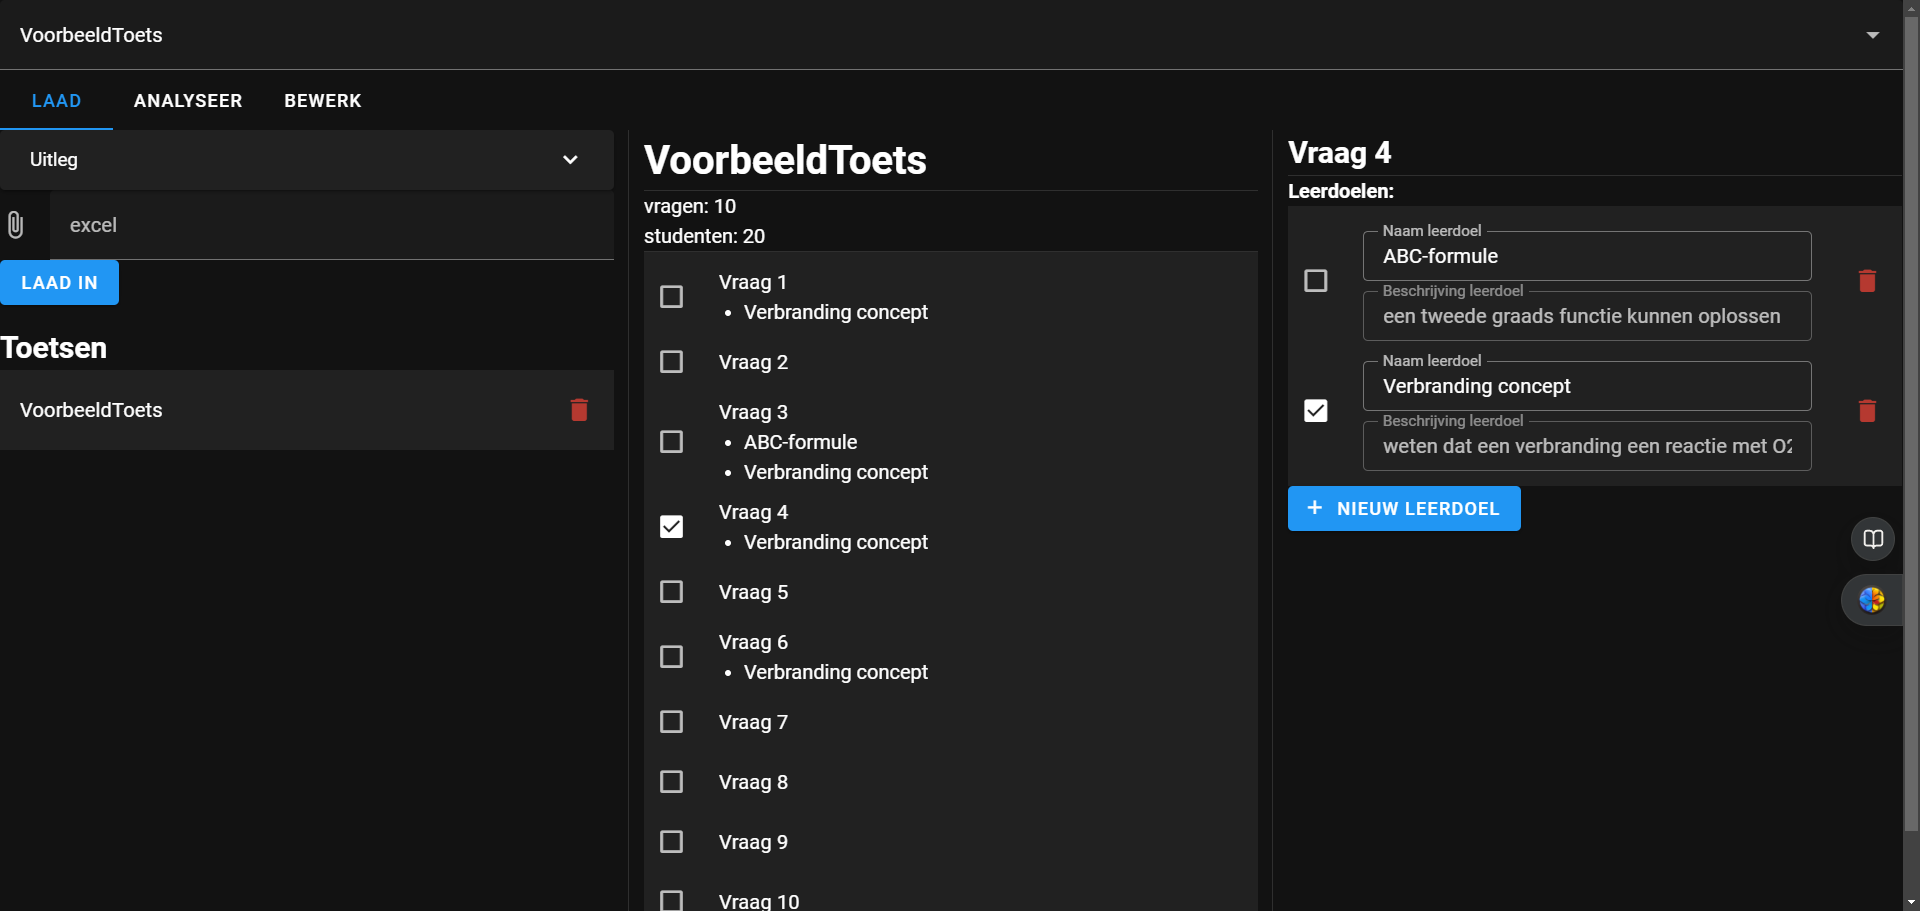
\includegraphics[width=1\linewidth]{./images/methoden/analyseren/ui/inlaad-pagina.png}
    \caption{Voorbeeld inlaadpagina}
    \label{fig:enter-label}
\end{figure}
\noindent In het \textbf{analyse scherm} moet voor een docent overzichtelijk weergegeven zijn welke vragen goed en minder goed gingen en de scores van de leerlingen. Hier moet ook te zien zijn welke vragen waarschijnlijk niet thuishoren in de toets, omdat de mensen met een hoog cijfer hem fout hebben, dit kan komen dat die leerlingen te ver doordenken en daardoor de vraag fout hebben. De vraag is of je die leerlingen wilt afstraffen voor het verder denken dan het juiste antwoord. \\
\\
Het is ook mogelijk om hier opvallende correlaties tussen vragen weer te geven. Hier kan bijvoorbeeld worden laten zien dat mensen die vraag 5 fout hebben ook vraag 8 fout hebben. Dan is het mogelijk dat er 2x om dezelfde kennis wordt gevraagd, iets wat een toetsresultaat minder betrouwbaar maakt, omdat de stof disproposioneel wordt getoetst (dit geld ook voor een hoge correlatie tussen 2 juist gemaakte vragen). \\
\\
Het kan ook mogelijk zijn om de correlaties tussen leerlingen te tonen om eventuele spiekers te vangen. Hierbij moet wel rekening gehouden worden met het feit dat 2 mensen met een hoog cijfer, waarschijnlijk beide dezelfde vragen goed en fout hebben. Deze coorelatie wordt wel interessant bij bijvoorbeeld 2 6.5'en en precies dezelfde fouten.\\
\\
Op \textbf{het bewerkscherm} kunnen bijvoorbeeld een aantal velden komen met de doelen van een docent. Bijvoorbeeld: een veld om het gewilde gemiddelde en de gewilde standaardeviatie in te stellen. Daarmee berekent hij dat een nieuwe formule. Hier kan ook worden of een lineare of non-lineare formule gebruikt wordt. Bij een non-lineare formule behoudt iedereen met een onvoldoende zijn onvoldoende, maar zijn die onvoldoendes minder hoog. \\
Hier kan ook op vraagniveau een scherm zijn om vragen eruit te gooien of half te laten meetellen, als blijkt dat ze wegnemen van de kennismeting van de toets.
% TODO: foto linear en non-linear
\end{multicols}
\pagebreak
\subsubsection{Enquete}
\begin{tabularx}{\linewidth}{ll}
    \textbf{Eigenaar: } & \textit{Jonathan en Joost} \\
    \textbf{Doel(en): } & 
        \makecell[tl]{
            $\bullet$ Inzicht krijgen in de mogelijkheid in de integratie van AI bij docenten op Het Amsterdams Lyceum \\
        } \\
    \textbf{Subvragen: } & 
        \makecell[tl]{
            $\bullet$ Hoe neem je een betrouwbare enquête? \\
            $\bullet$ Hoe zorg je ervoor dat mensen jouw enquête willen invullen? \\
        }\\
    \textbf{Kader(s): } & 
        \makecell[tl]{
            $\bullet$ TODO
        }\\
    \parbox[t]{3cm}{\raggedright \textbf{Geschatte  tijdskosten:} } & 20 uur \\
\end{tabularx}
\begin{multicols}{2}
Om te testen of docenten uberhaupt open staan voor een ai model hebben we een enquête verstuurd naar alle docenten van Het Amsterdams Lyceum. 
Om een betrouwbare enquête te maken moet je als eerste het doel van de enquête duidelijk hebben. In ons onderzoek waren dat de volgende:
\begin{minipage}{\linewidth}
\begin{itemize}
    \item target voor ons programma stellen
    \item mogelijke acceptatie in kaart brengen
\end{itemize}
\end{minipage}
Daarnaast moet elke vraag ook een duidelijk doel hebben, anders is het mogelijk dat je 2x dezelfde vraag stelt of naar informatie gaat vrageb niet niet relevant is.\\
Ten slotte moesten we bij elke vraag nagaan of de vraag op verschillende manieren geinterpreteerd kan worden.\\
Dit waren de vragen die we hebben bedacht:
% TODO: verklaringen toevoegen
\end{multicols}%
\begin{longtable}{p{0.5\linewidth}|p{0.25\linewidth}|p{0.25\linewidth}}
    Vraag & Doel & Verklaring \\
    \endhead
    \hline 
    \begin{minipage}[t]{\linewidth}
        \textbf{1. Wat is uw vakgebied? (Indien meerdere, kies vak met meeste uren a.u.b.) }
        \hspace{4em} Vakken        
    \end{minipage} & kunnen filtreren op vakgebied en vakgroep ($\alpha, \beta, \gamma$) & \\
    \hline 
    \begin{minipage}[t]{\linewidth}
        \textbf{2. Hoeveel jaar bent u al docent? }
        \begin{itemize}
            \item 1-5 jaar
            \item 5-10 jaar
            \item Meer dan tien jaar
            \item Minder dan één jaar
        \end{itemize}
    \end{minipage} & kunnen filtreren op lesgeef ervaring & \\
    \hline 
    \begin{minipage}[t]{\linewidth}
        \textbf{3. Bent u bekend met het concept van (generatieve) AI? }
        \begin{itemize}
            \item Ja, ik ben goed op de hoogte
            \item Ja, ik heb er wel eens over gehoord
            \item Nee, ik ben niet bekend met deze technologie
        \end{itemize}
    \end{minipage} & kunnen filtreren op ai ervaring & \\
    \hline 
    \begin{minipage}[t]{\linewidth}
        \textbf{4. Wat zouden voor u redenen zijn om AI te gebruiken voor het nakijken van proefwerken? (Meerdere antwoorden mogelijk) }
        \begin{itemize}
            \item Tijdbesparing
            \item Objectiviteit in de beoordeling
            \item Vermindering van de werkdruk
            \item Snelheid van de terugkoppeling naar studenten
            \item Betere nauwkeurigheid
            \item Ik zou nooit overwegen AI hierbij te gebruiken
            \item Anders: \textit{zelf invullen}

        \end{itemize}
    \end{minipage} & weten wat het hoofddoel moet zijn van ons programma en wat waar we minder aandacht aan kunnen besteden & \\
    \hline 
    \begin{minipage}[t]{\linewidth}
        \textbf{5. Wat zijn uw belangrijkste zorgen bij het gebruik van AI voor het nakijken van proefwerken? (Tot 4 antwoorden mogelijk) }
        \begin{itemize}
            \item Gebrek aan menselijke empathie in de beoordeling
            \item Mogelijke technische fouten
            \item Onvoldoende aandacht voor subjectieve antwoorden
            \item Data- en privacykwesties van studenten
            \item Oneerlijke of bevooroordeelde beoordelingen
            \item Afhankelijkheid van technologie
            \item Anders: \textit{zelf invullen}
        \end{itemize}
    \end{minipage} & weten waar we op moeten focussen en wrten of bepaalde problemen een grote bottleneck zullen zijn voor de acceptatie van ons programma voor docenten & \\
    \hline 
    \begin{minipage}[t]{\linewidth}
        \textbf{6. Denkt u dat AI zelfstandig toetsen zou kunnen nakijken}
        \begin{itemize}
            \item Ja
            \item Nee
            \item Weet ik niet
        \end{itemize}
    \end{minipage} & weten hoe positief docenten in een mogelijkheid zijn en om te vergelijken met vakgebied en lesgeef ervaring & \\
    \hline 
    \begin{minipage}[t]{\linewidth}
        \textbf{7. Hoeveel leerlingen trekken uw beoordeling per toets - terecht of niet - in twijfel? (Een getal)}\\
        \vspace{4em} Zelf een getal invullen
    \end{minipage} & 
        \begin{minipage}[t]{\linewidth}
            Een objectief target halen waarmee we ons programma kunnen vergelijken:\\ 
            meer oneens is slechter of te streng naar gekeken \\ 
            te weinig is te makkelijk nagekeken 
        \end{minipage}
        & \\
    \hline 
    \begin{minipage}[t]{\linewidth}
        \textbf{8. Welke invloed denkt u dat de inzet van AI kan hebben op de relatie tussen docent en student? (Open vraag) }\\
        \vspace{4em} Zelf een getal invullen

    \end{minipage} & Als docenten nog wat kwijt willen kunnen ze dat hier doen, misschien staat er wat interessants tussen & \\
\end{longtable}
\begin{multicols}{2}
Ons 2e doel van dit onderdeel was \textbf{Hoe zorg je ervoor dat mensen jouw enquête willen invullen?}.\\
Uit ons kleine omgevingsonderzoek blijkt dat docenten van Het Amsterdams Lyceum niet vaak reageren op (onbelangrijke) mail. Een score van 30\% zou al aan de hoge kant zijn. We hebben een zakelijk mailtje proberen samen te stellen die ervoor zorgt dat docenten wilden reageren. \\
\fbox{\begin{minipage}{\linewidth}
    
Geachte docenten van Het Amsterdams Lyceum,\\
\\
In het kader van ons profielwerkstuk, maken wij een programma dat dat toetsen kan inscannen, nakijken en analyseren. \\
Daarnaast zijn we geïnteresseerd in hoe docent denken over het nakijken met AI, hierbij zouden wij graag uw hulp willen.\\
\\
https://forms.office.com/e/j5cYFrAy7p 
\\
Hoogachtend,\\
\\
Joost Koch & Jonathan Wijker
\end{minipage}}
Op dit mailtje hebben we 22 reacties gekregen. Dat vonden wij redelijk tegenvallen.
Een rede voor deze teleurstellende respons zou kunnen zijn dat we de mail verstuurd hebben op donderdag 17 oktober. Dat was de donderdag voor de activiteitenweek, waardoor docenten met uitzicht op een vakantie misschien geen zin hadden in het invullen van een PWS-enquête.\\
\\
Daarna hebben de gekeken wat het ideale moment zou zijn voor een docent om zin te hebben in het invullen van een enquête. Toen kwamen we na overleg met diverse docenten erachter dat de week voor de toetsweek het rustigst is, want de meeste docenten hebben alle lesstof al behandeld, geen toetsen om na te kijken en hebben de toetsen en SE's al af en ingelevert.  \\
\\
We hebben ons tweede mailtje op de maandag voor de toetsweek gestuurd. We hebben ook de docenten extra proberen te vleien door duidelijk aan te geven dat het weinig tijd kost en dat we weten hoe druk docenten het eigenlijk hebben.
\fbox{\begin{minipage}{\linewidth}
    
Geachte docent,

Onlangs hebben wij u een enquête gestuurd en we hebben al wat reacties mogen ontvangen, bedankt daarvoor.
We snappen dat u het komende tijd druk heeft met de toetsweek, maar hopen dat u komende week ergens een gaatje van 2-3 minuten kunt vinden om alsnog onze enquête in te vullen. Dit zouden we erg waarderen!
 
https://forms.office.com/e/j5cYFrAy7p


Hoogachtend,
 
Joost Koch & Jonathan Wijker
\end{minipage}}
Dit leverde 28 extra responses op, waardoor we op een totaal van 50 zitten. Dit is statistisch gezien goed genoeg om iets over de meningen van de docenten te zeggen op Het Amsterdams Lyceum. \\
% TODO: deze claim over statistiek met bron
We moeten er wel rekening mee houden dat sommige secties misschien minder zullen hebben gereageerd, waardoor ons resultaat over die sectie minder betrouwbaar zal zijn.\\
\\
% TODO: tijden checken (gaan we)
Voor het analyseren gaan we Google Sheet pivot tables gebruiken om snel verbanden tussen de data te zien. Ook zullen we kijken of ChatGPT of Google Gemini relevante ontdekkingen kunnen doen in de data. 


\end{multicols}



\section{Resultaten}
\subsection{Inscannen}

\subsection{Nakijken}

\subsection{Analyseren}

\subsection{Enquête}


\begin{table}[h!]
\centering
\resizebox{\textwidth}{!}{%
\begin{tabular}{lcccc}
\toprule
\textbf{Hoeveel jaar bent u al docent?} & 
\textbf{Ja} & 
\textbf{Een beetje} & 
\textbf{Nee} & 
\textbf{Total} \\ 
\midrule
1-5 jaar          & 4 & 4 & 0 & 8  \\
5-10 jaar         & 5 & 4 & 0 & 9  \\
Meer dan tien jaar & 13 & 16 & 1 & 30 \\
Minder dan één jaar & 1 & 1 & 0 & 2  \\
\midrule
\textbf{Grand Total} & \textbf{23} & \textbf{25} & \textbf{1} & \textbf{49} \\
\bottomrule
\end{tabular}%
}
\caption{Samenvatting van bekendheid met generatieve AI onder docenten.}
\label{tab:docenten_technologie}
\end{table}

\begin{table}[h!]
\centering
\resizebox{\textwidth}{!}{%
\begin{tabular}{lcccc}
\toprule
\textbf{Hoeveel jaar bent u docent?} & 
\textbf{Ja (\%)} & 
\textbf{Nee (\%)} & 
\textbf{Weet ik niet (\%)} & 
\textbf{Total (\%)} \\ 
\midrule
1-5 jaar          & 37.50 & 50.00 & 12.50 & 100.00 \\
5-10 jaar         & 44.44 & 33.33 & 22.22 & 100.00 \\
Meer dan tien jaar & 23.33 & 40.00 & 36.67 & 100.00 \\
Minder dan één jaar & 50.00 & 50.00 & 0.00 & 100.00 \\
\midrule
\textbf{Grand Total} & \textbf{28.57} & \textbf{40.82} & \textbf{30.61} & \textbf{100.00} \\
\bottomrule
\end{tabular}%
}
\caption{Percentageverdeling van vertrouwen met nakijken door AI onder docenten.}
\label{tab:docenten_percentage}
\end{table}
\begin{table}[h!]
\centering
\resizebox{\textwidth}{!}{%
\begin{tabular}{lcc}
\toprule
\textbf{Hoeveel jaar bent u al docent?} & 
\textbf{Gemiddeld aantal leerlingen} & 
\textbf{Aantal docenten} \\ 
\midrule
1-5 jaar          & 3.375 & 8 \\
5-10 jaar         & 1.222 & 9 \\
Meer dan tien jaar & 1.862 & 30 \\
Minder dan één jaar & 7.500 & 2 \\
\midrule
\textbf{Grand Total} & \textbf{2.229} & \textbf{49} \\
\bottomrule
\end{tabular}%
}
\caption{Gemiddelde van het aantal leerlingen dat de beoordeling van docenten in twijfel trekt, per ervaringscategorie.}
\label{tab:gemiddelde_twijfel}
\end{table}


\section{conclusie}
\subsection{Inscannen}

\subsection{Nakijken}

\subsection{Analyseren}

\subsection{Enquete}


\section{Discussie}
\subsection{Foutenanalyse}
\subsubsection{Inscannen}

\subsubsection{Nakijken}

\subsubsection{Analyseren}

\subsubsection{Enquête}



\subsection{vervolgonderzoek}
\section{Samenvatting onderzoek}

\section{Referenties}
\section{Bijlagen}
\end{document}
